\documentclass[10pt,pdf,hyperref={unicode}]{beamer}

\usetheme[progressbar=frametitle]{metropolis}
\usepackage{booktabs}
\usepackage[scale=2]{ccicons}
\usepackage{pgfplots}
\usepgfplotslibrary{dateplot}
\usepackage{xspace}
\newcommand{\themename}{\textbf{\textsc{metropolis}}\xspace}
\usepackage{multicol}
\usepackage[T2A]{fontenc}
\usepackage[utf8]{inputenc}
\usepackage{listings}
\usepackage{hyperref}
\usepackage{textcomp}


\usetheme{Pittsburgh}
\usecolortheme{seahorse}
\definecolor{light-gray}{gray}{0.90}


\lstset{
  language=C++,                % choose the language of the code
  basicstyle=\linespread{1.1}\ttfamily,
  columns=fixed,
  fontadjust=true,
  basewidth=0.5em,
  keywordstyle=\color{blue}\bfseries,
  commentstyle=\color{gray},
  stringstyle=\ttfamily\color{orange!50!black},
  showstringspaces=false,
  numbersep=5pt,
  numberstyle=\tiny\color{black},
  numberfirstline=true,
  stepnumber=1,                   % the step between two line-numbers.        
  numbersep=10pt,                  % how far the line-numbers are from the code
  backgroundcolor=\color{black!2},  % choose the background color. You must add \usepackage{color}
  showstringspaces=false,         % underline spaces within strings
  captionpos=b,                   % sets the caption-position to bottom
  breaklines=true,                % sets automatic line breaking
  breakatwhitespace=true,         % sets if automatic breaks should only happen at whitespace
  xleftmargin=.2in,
  extendedchars=\true,
  keepspaces = true,
}

\newcommand\upquote[1]{\textquotesingle#1\textquotesingle}


\title{Структуры данных в C++}
\author{Бирюков В. А.} 
\date{\today}
\begin{document}

\begin{frame}
\titlepage
\end{frame} 

\begin{frame}[fragile]
\frametitle{Структуры данных} 
\begin{itemize}
\item Статический массив
\item Динамический массив
\item Связный список
\item Дерево
\item Хеш-таблица
\end{itemize}
\end{frame}

\section{Статический массив} 

\begin{frame}[fragile]
\frametitle{Статический массив} 
\begin{lstlisting}
int a[10] = {10, 20, 30, 40, 50};
int n = 5;
\end{lstlisting}
\begin{center}
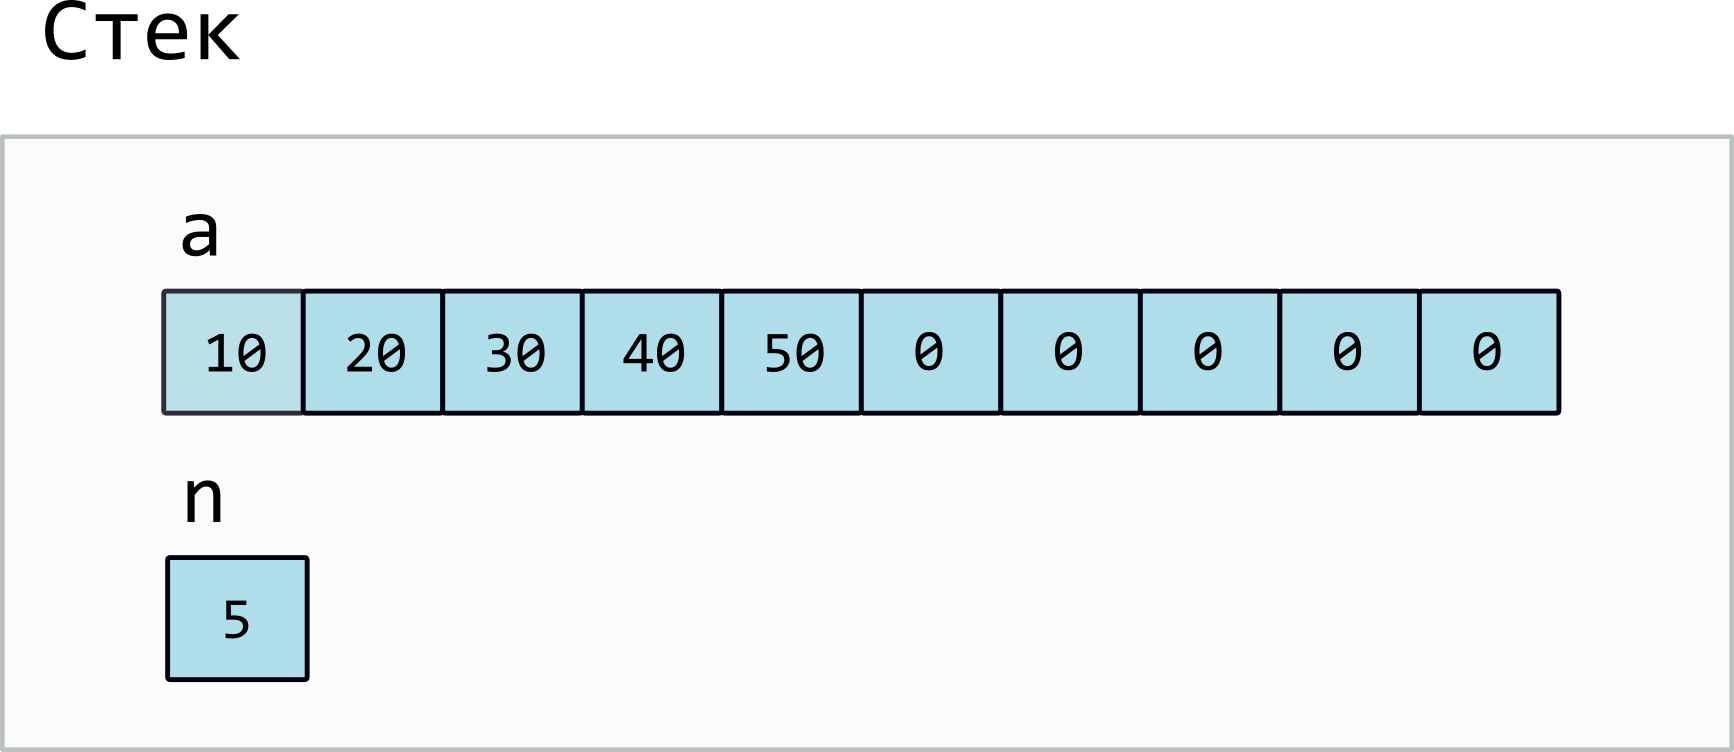
\includegraphics[scale=0.6]{images/static_array/static_array.png}
\end{center}
\end{frame}


\begin{frame}[fragile]
\frametitle{Статический массив} 
\begin{lstlisting}
std::array<int, 10> a {10, 20, 30, 40, 50};
int n = 5;
\end{lstlisting}
\begin{center}
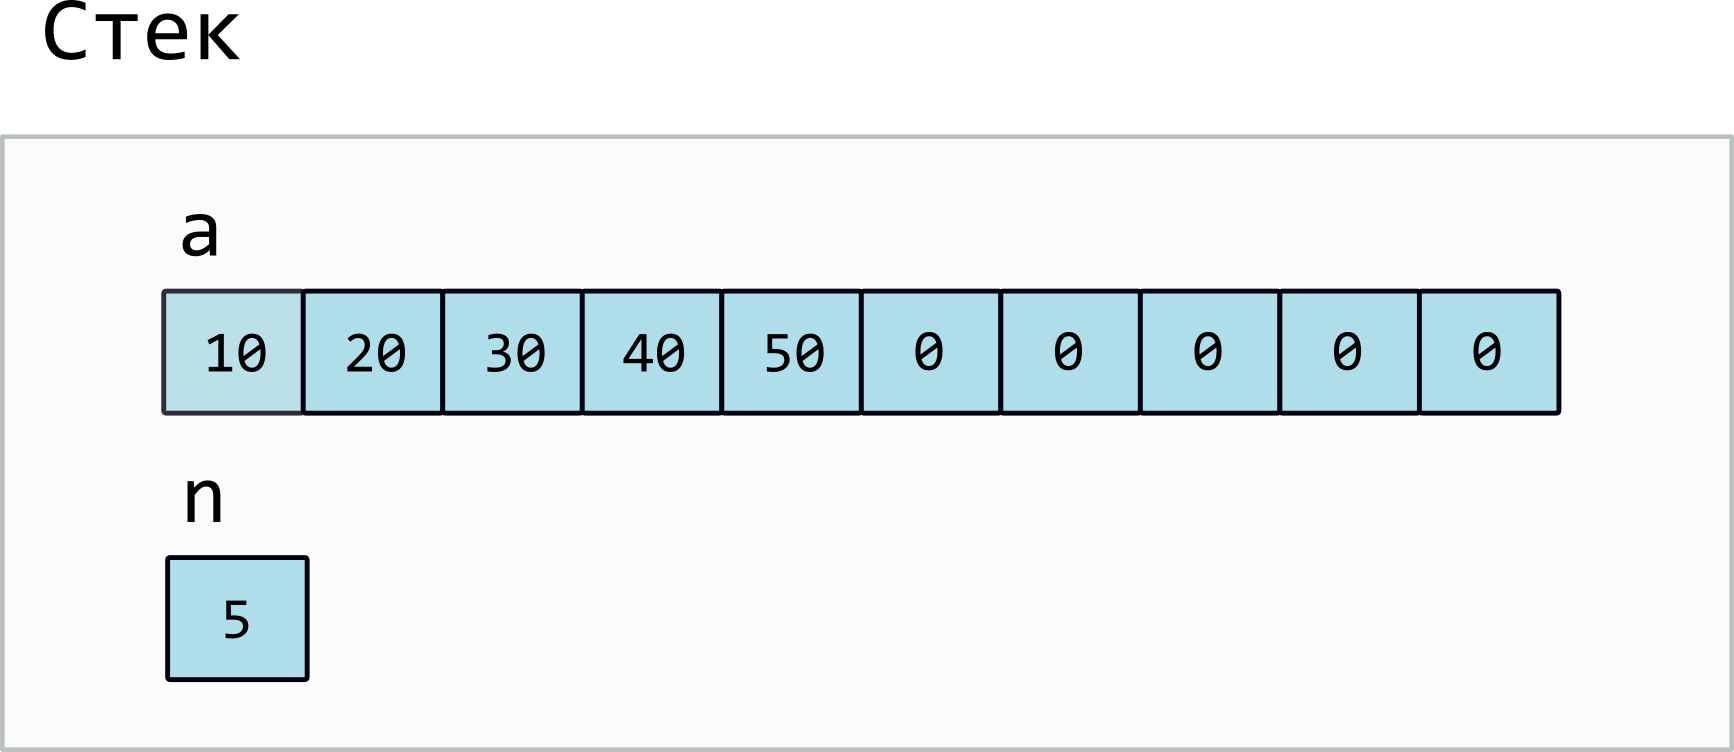
\includegraphics[scale=0.6]{images/static_array/static_array.png}
\end{center}
\end{frame}


\section{Динамический массив} 

\begin{frame}[fragile]
\frametitle{Динамический массив в языке C} 
\begin{lstlisting}
#include <stdlib.h>
...
int n = 5;
int* p = (int*)malloc(n * sizeof(int));
for (int i = 0; i < n; ++i)
    p[i] = (i + 1) * 10;
\end{lstlisting}
\begin{center}
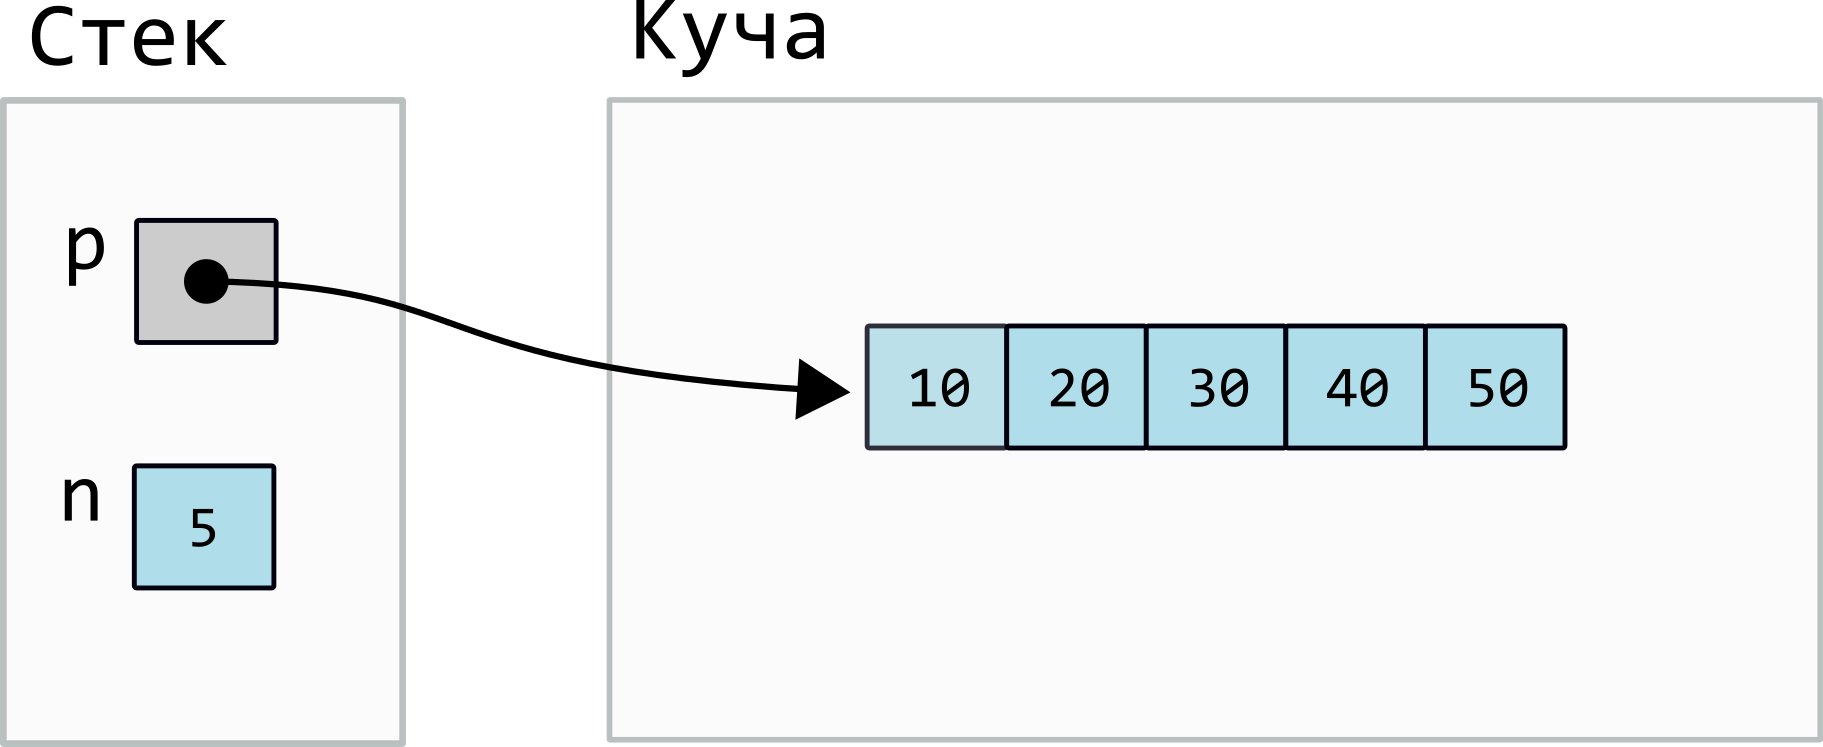
\includegraphics[scale=0.6]{images/dynamic_array/dynamic_array.png}
\end{center}
\end{frame}


\begin{frame}[fragile]
\frametitle{Динамический массив в языке C++ с помощью \texttt{new}} 
\begin{lstlisting}
int* p = new int[5] {10, 20, 30, 40, 50};
int n = 5;
\end{lstlisting}
\begin{center}
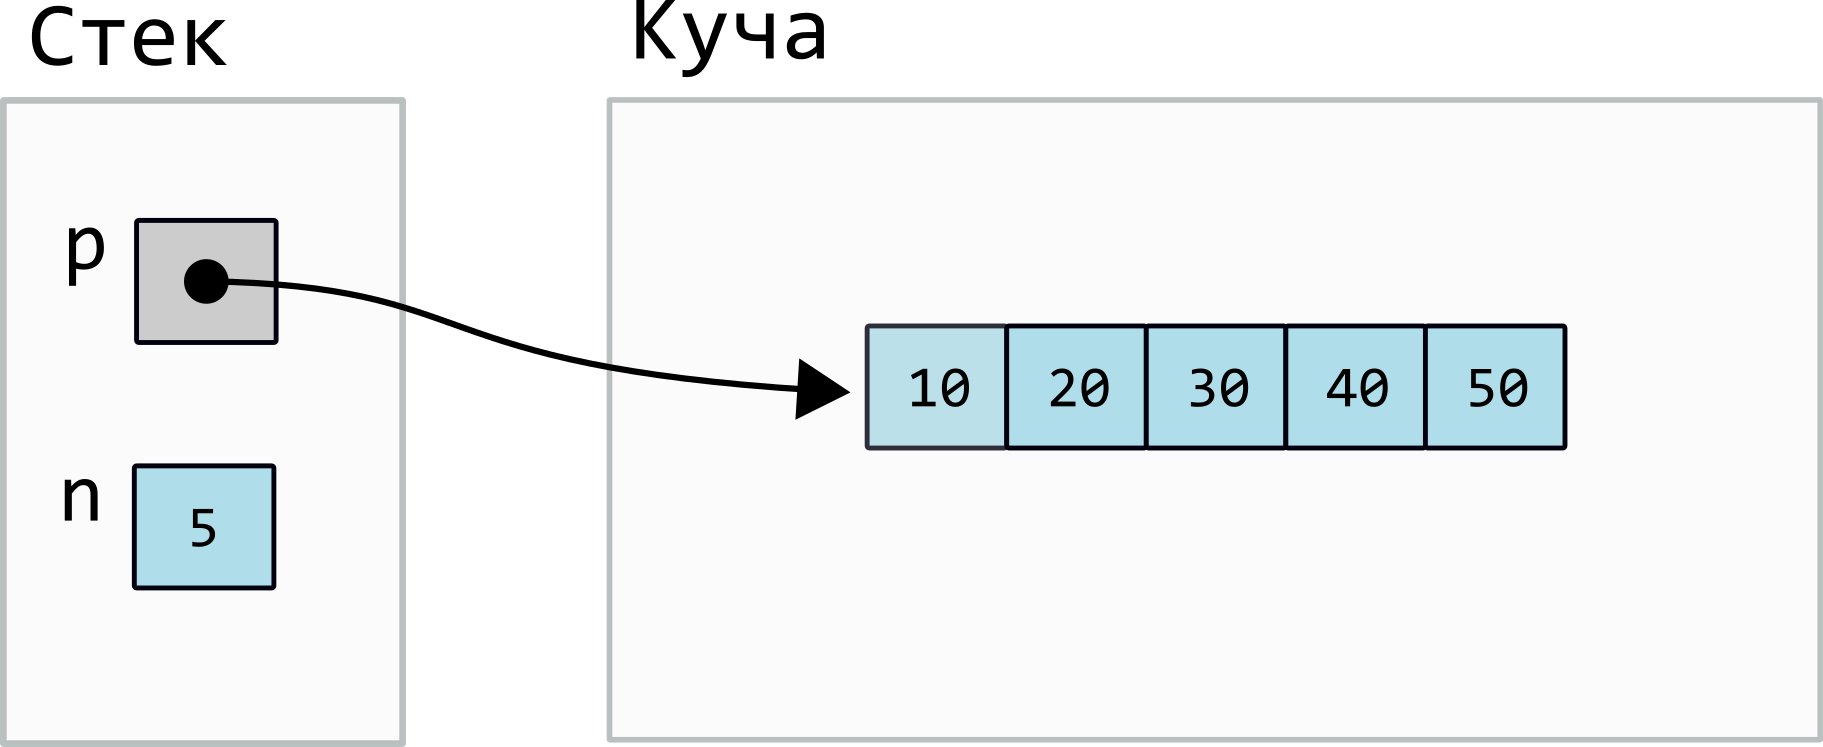
\includegraphics[scale=0.6]{images/dynamic_array/dynamic_array.png}
\end{center}
\end{frame}


\begin{frame}[fragile]
\frametitle{Добавим ещё один элемент в динамический массив} 
\begin{lstlisting}
int* p = new int[5] {10, 20, 30, 40, 50};
int n = 5;
int* q = new int[n + 1];
\end{lstlisting}
\begin{center}
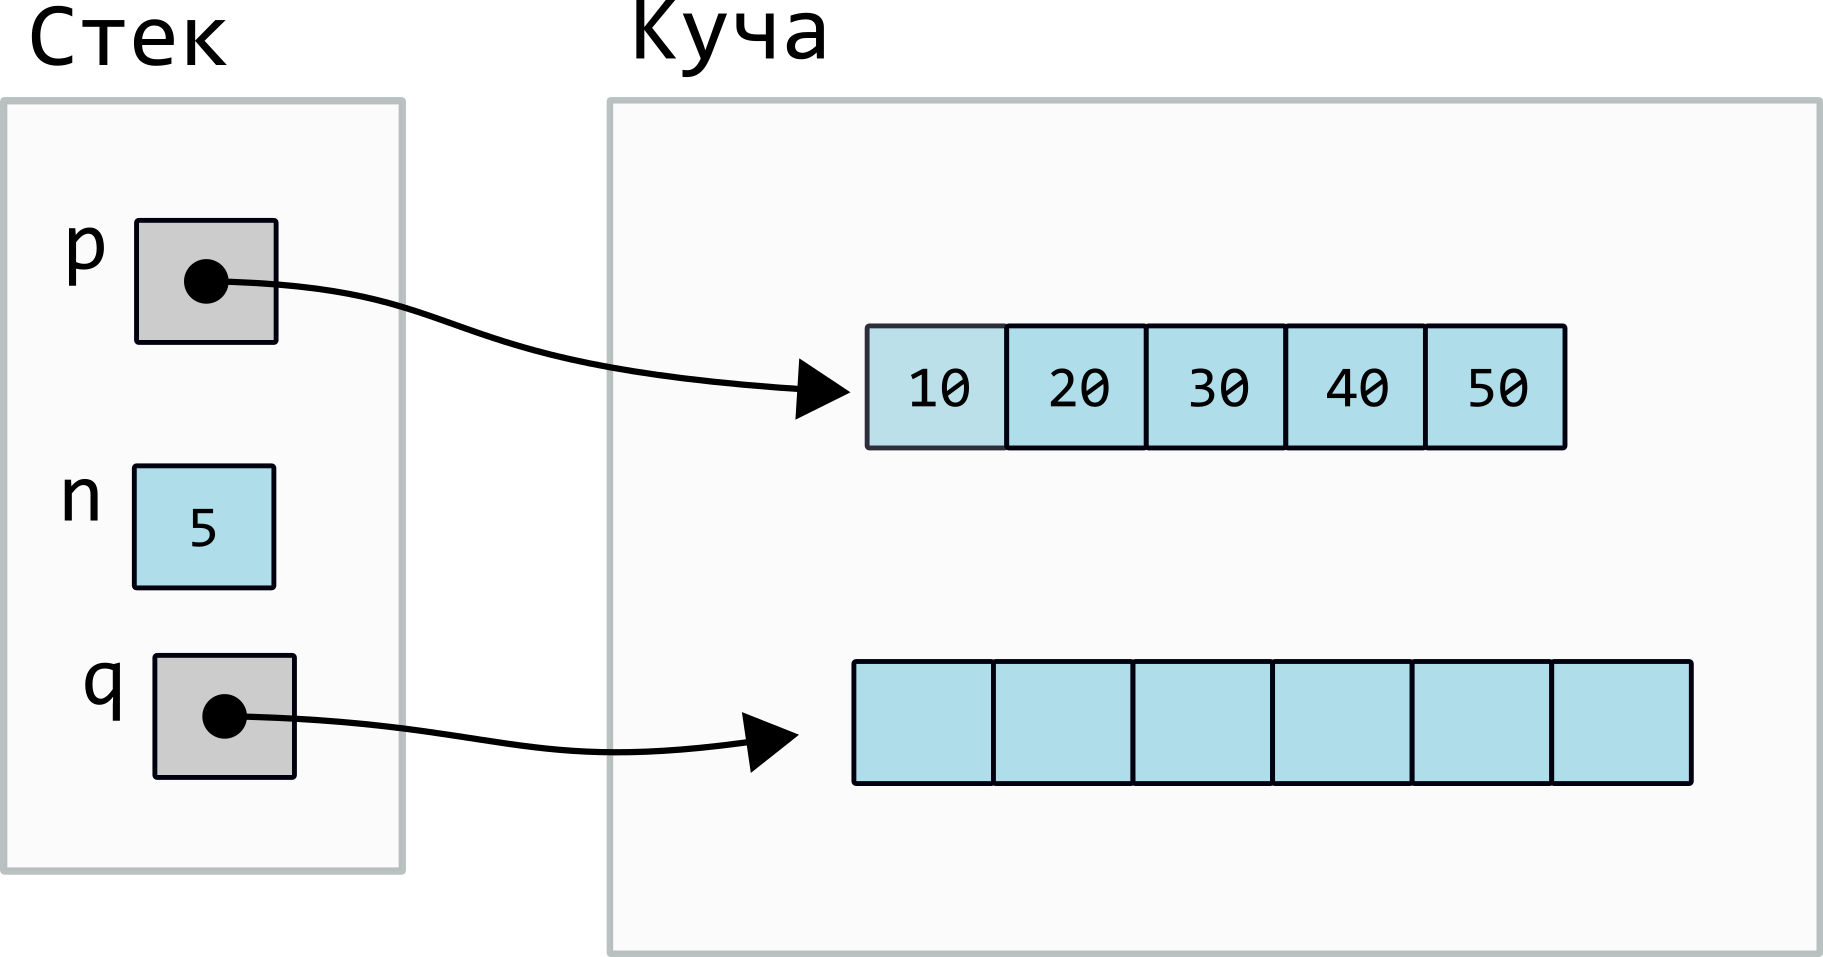
\includegraphics[scale=0.6]{images/dynamic_array/dynamic_array_add_one1.png}
\end{center}
\end{frame}

\begin{frame}[fragile]
\frametitle{Добавим ещё один элемент в динамический массив} 
\begin{lstlisting}
for (int i = 0; i < n; ++i)
    q[i] = p[i];
q[n] = 60;
\end{lstlisting}
\begin{center}
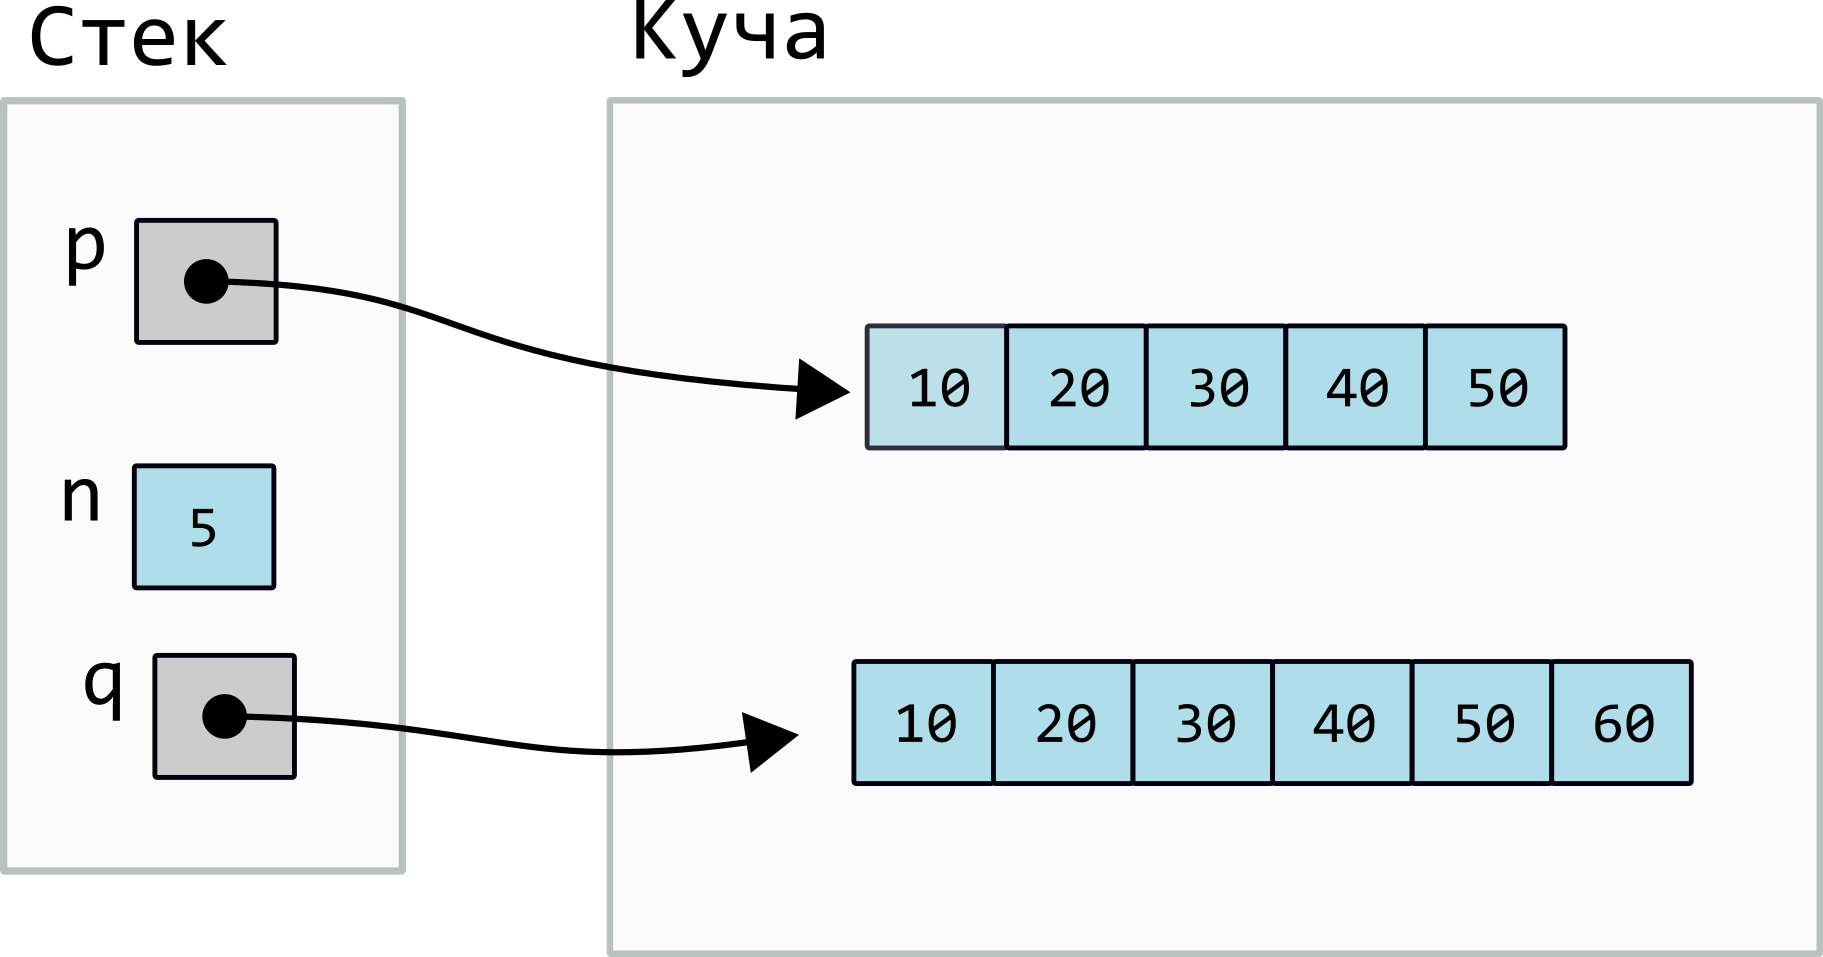
\includegraphics[scale=0.6]{images/dynamic_array/dynamic_array_add_one2.png}
\end{center}
\end{frame}

\begin{frame}[fragile]
\frametitle{Добавим ещё один элемент в динамический массив} 
\begin{lstlisting}
delete p;
p = q;
n += 1;
\end{lstlisting}
\begin{center}
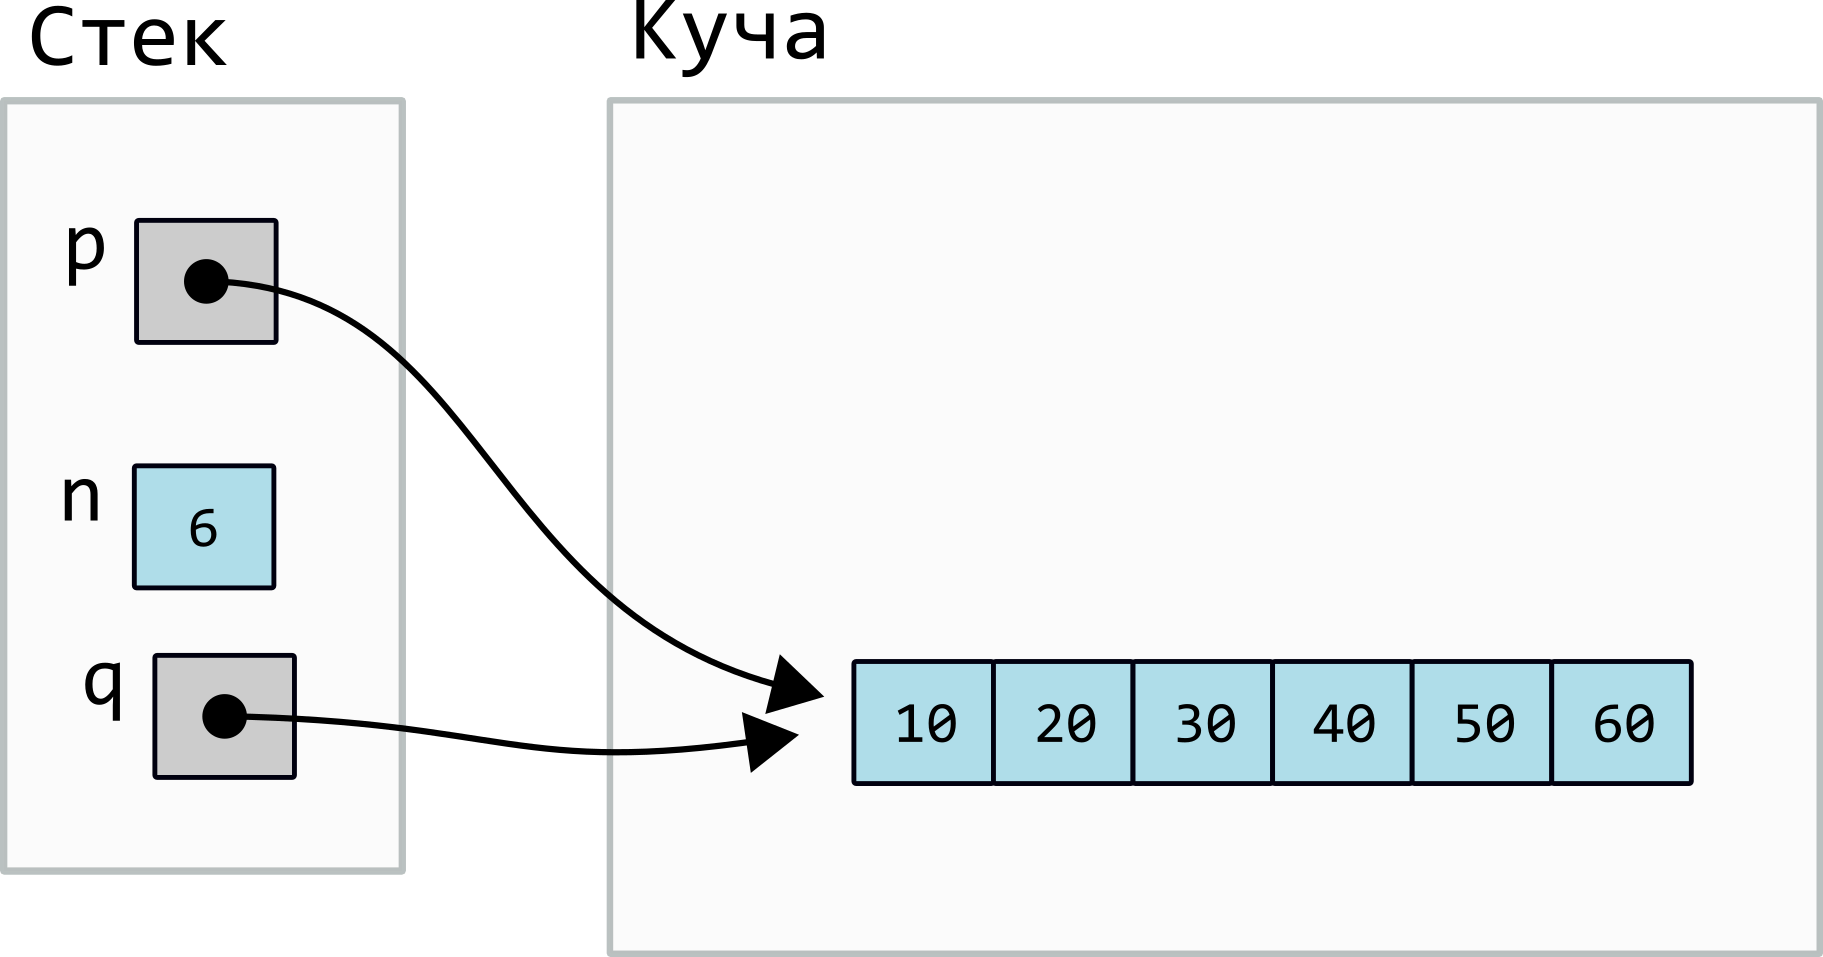
\includegraphics[scale=0.6]{images/dynamic_array/dynamic_array_add_one3.png}
\end{center}
\end{frame}

\begin{frame}[fragile]
\frametitle{Добавим ещё один элемент в динамический массив} 
\begin{itemize}
\item Предположим, что мы захотели добавить в динамический массив ещё 100 элементов.
Тогда при каждом добавлении элемента мы будем должны выделять в куче массив на один элемент больше и переписывать весь массив в новое место. 
Вычислительная сложность добавления $N$ элементов в такой массив будет равна $O(N^2)$.
\item Предположим, что мы захотели удалить 1 элемент из конца массива. Тогда нам тоже придётся перевыделять память, хотя без этого можно обойтись.
\end{itemize}
\end{frame}


\begin{frame}[fragile]
\frametitle{Вместимость} 
\begin{lstlisting}
int* p = new int[5] {10, 20, 30, 40, 50};
int size = 5;
int cap = 5;
\end{lstlisting}
\begin{center}
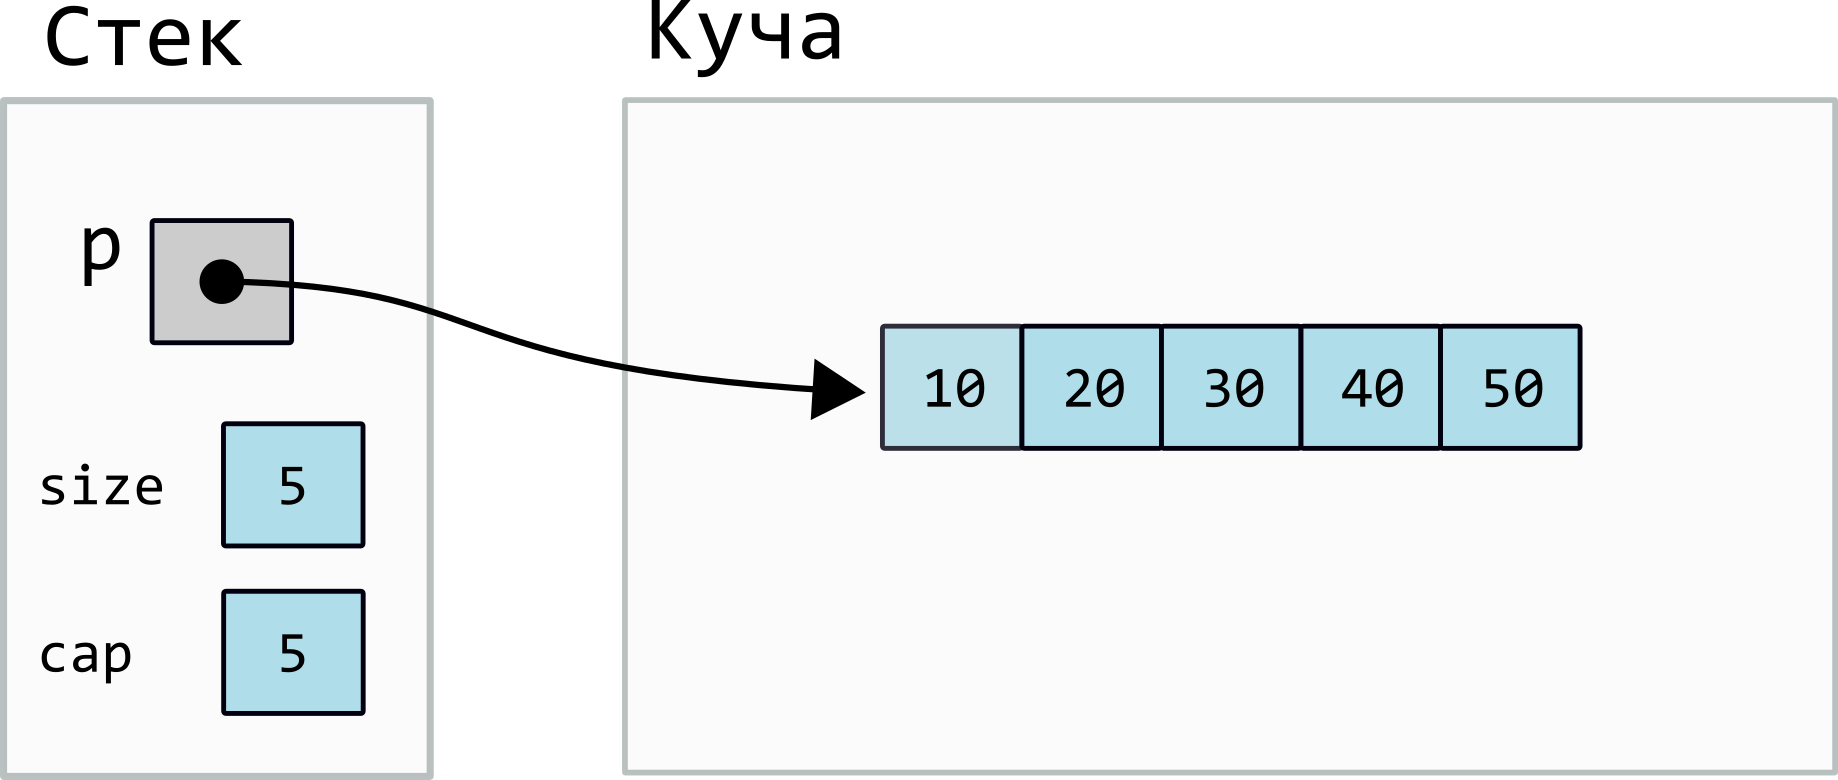
\includegraphics[scale=0.6]{images/dynamic_array/dynamic_array_cap.png}
\end{center}
\end{frame}


\begin{frame}[fragile]
\frametitle{Добавление элемента} 
\begin{lstlisting}
int* q = new int[2 * n];
for (int i = 0; i < size; ++i)
    q[i] = p[i];
q[size]++;
\end{lstlisting}
\begin{center}
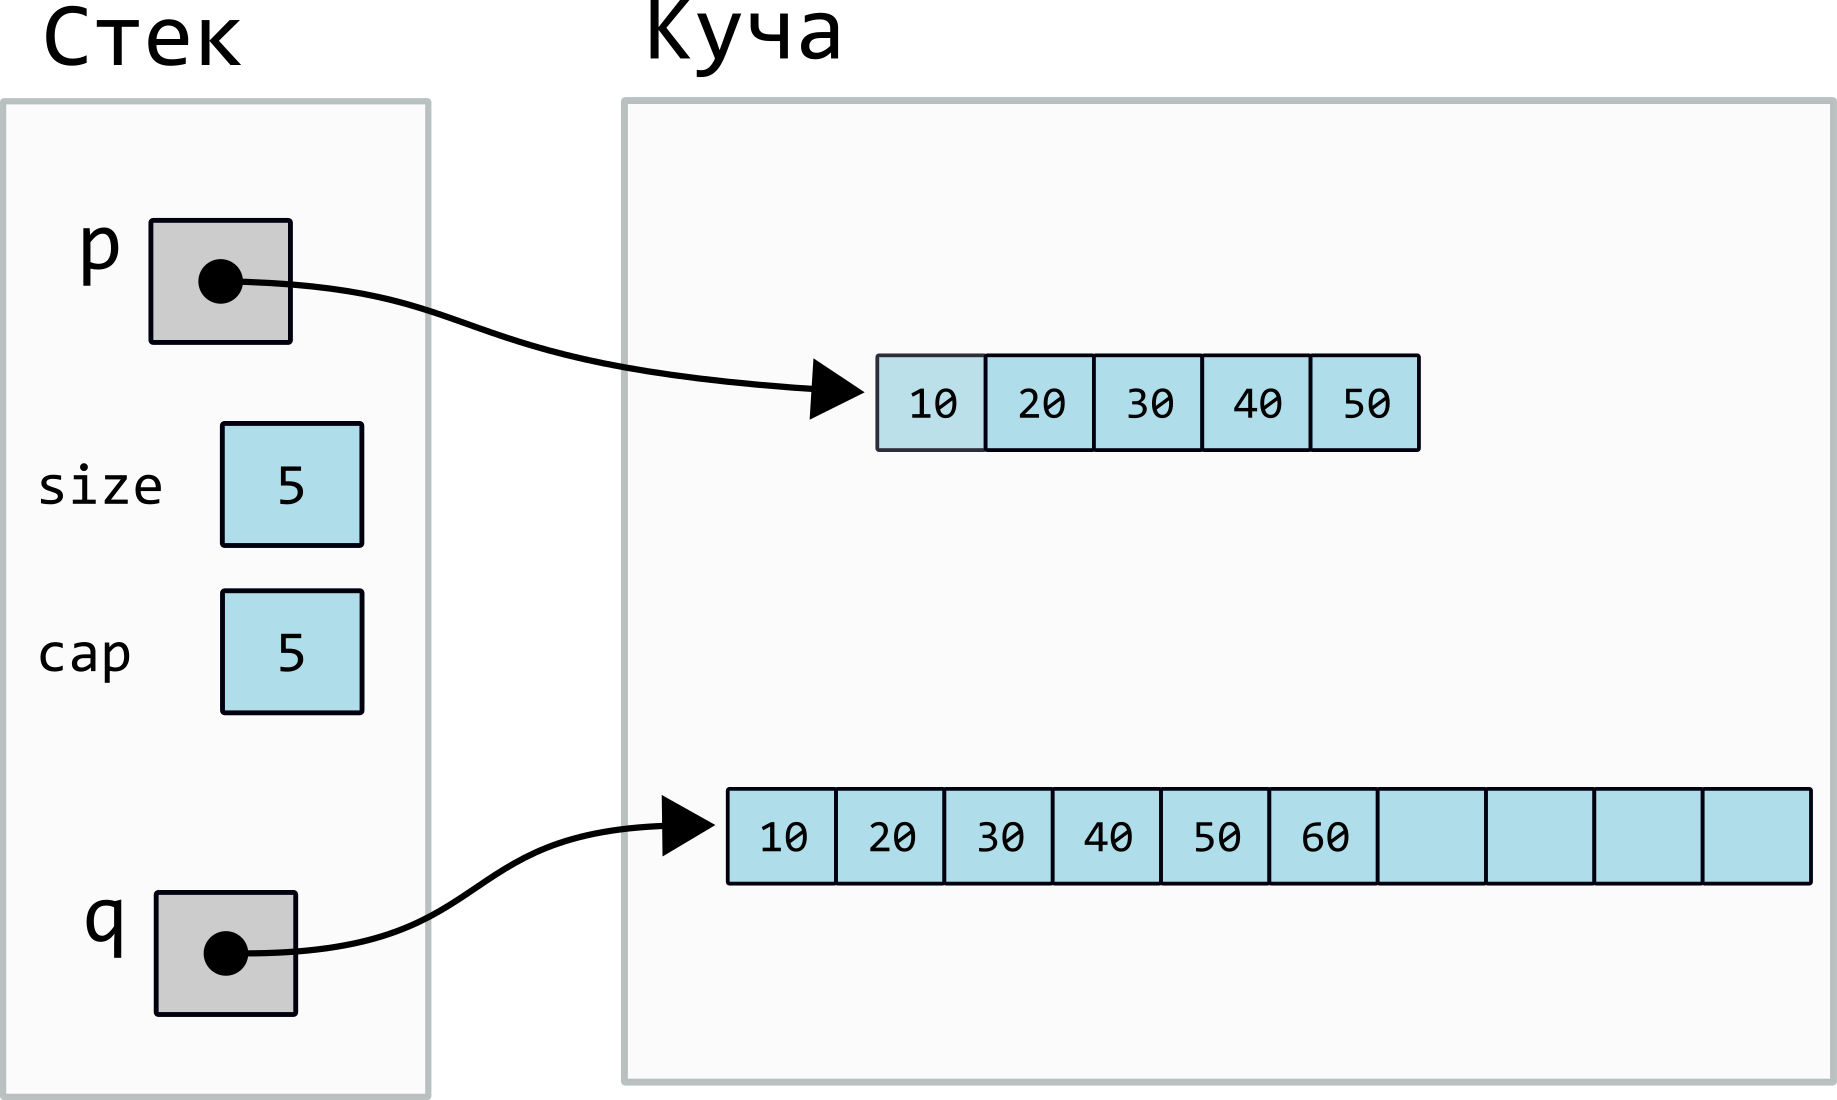
\includegraphics[scale=0.6]{images/dynamic_array/dynamic_array_cap_add_one1.png}
\end{center}
\end{frame}


\begin{frame}[fragile]
\frametitle{Добавление элемента} 
\begin{lstlisting}
delete p;
p = q;
size += 1;
cap *= 2;
\end{lstlisting}
\begin{center}
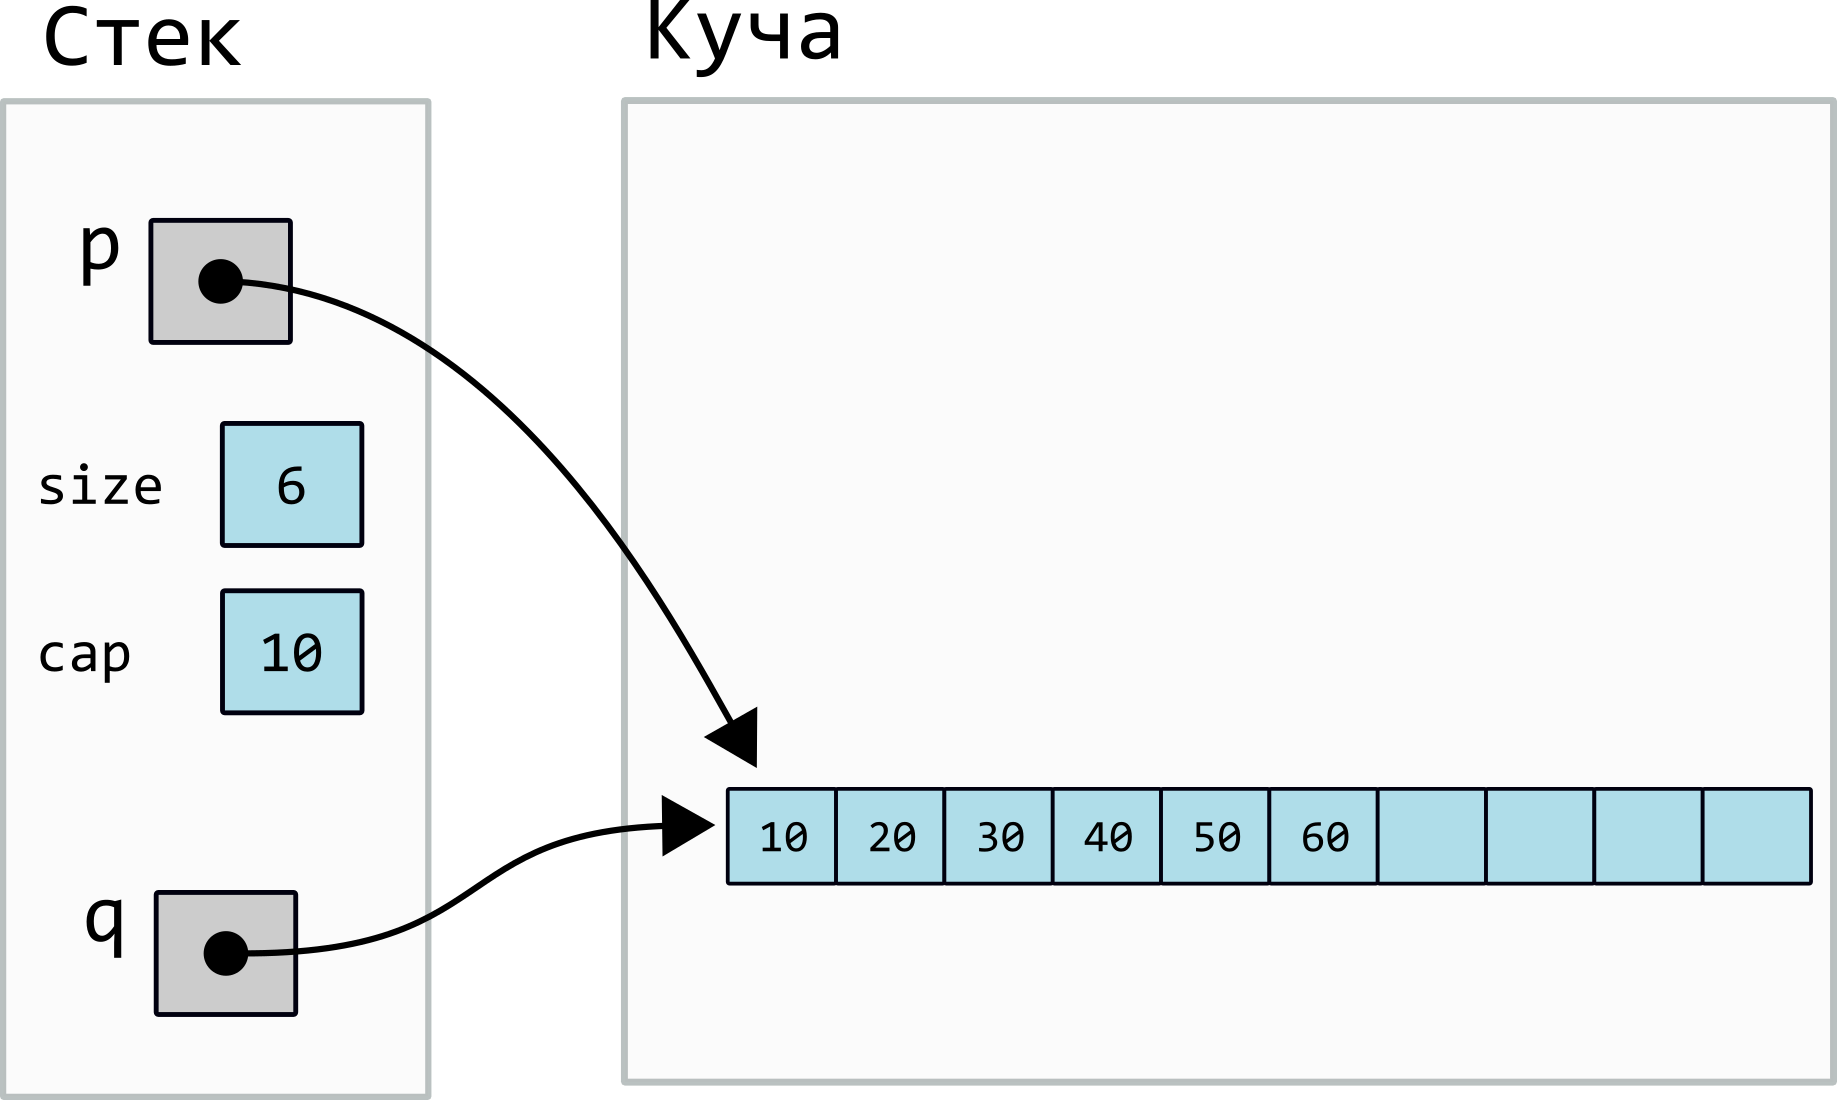
\includegraphics[scale=0.6]{images/dynamic_array/dynamic_array_cap_add_one2.png}
\end{center}
\end{frame}


\begin{frame}[fragile]
\frametitle{Добавление элемента} 
\begin{center}
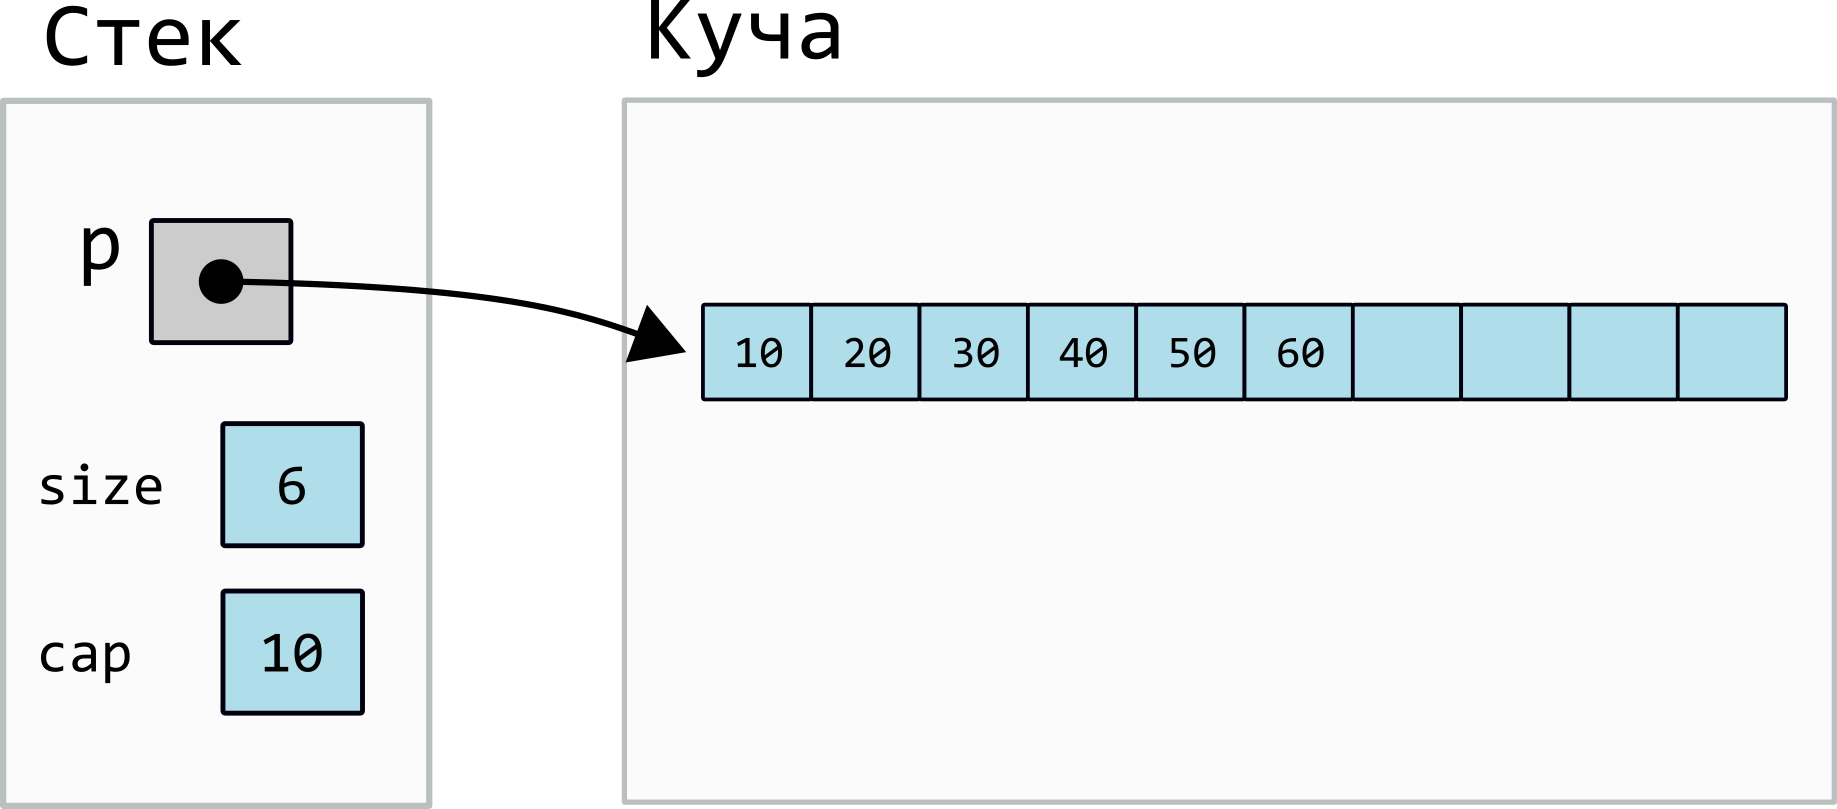
\includegraphics[scale=0.6]{images/dynamic_array/dynamic_array_cap_add_one3.png}
\end{center}
\end{frame}

\begin{frame}[fragile]
\frametitle{Добавление ещё одного элемента} 
\begin{center}
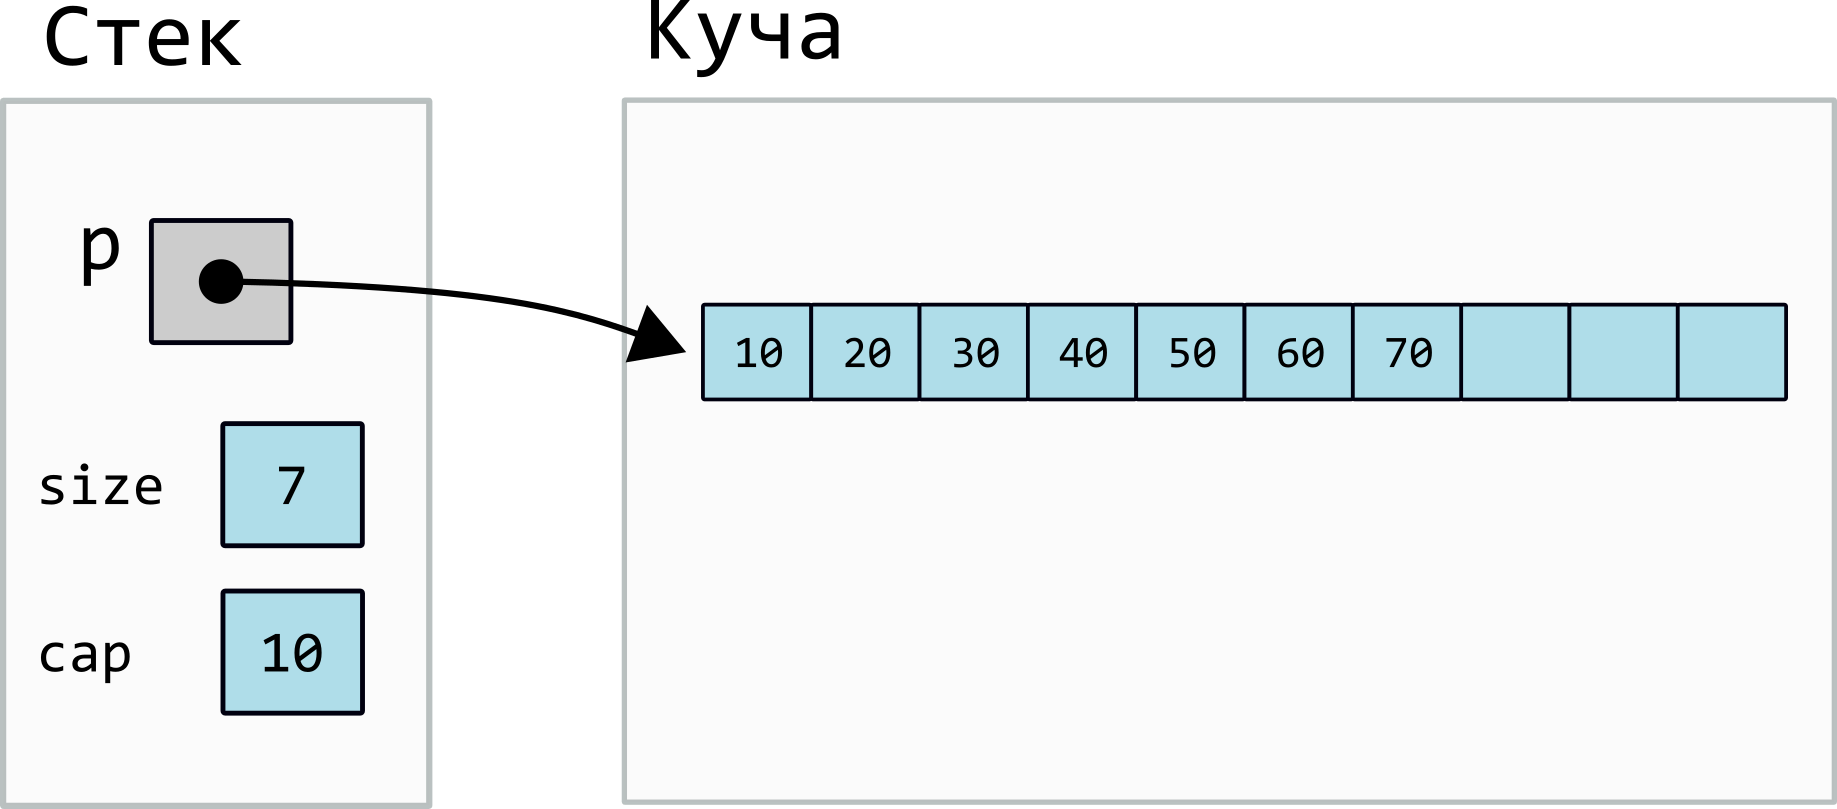
\includegraphics[scale=0.6]{images/dynamic_array/dynamic_array_cap_add_one4.png}
\end{center}
\end{frame}


\begin{frame}[fragile]
\frametitle{Удаление элементов} 
\begin{center}
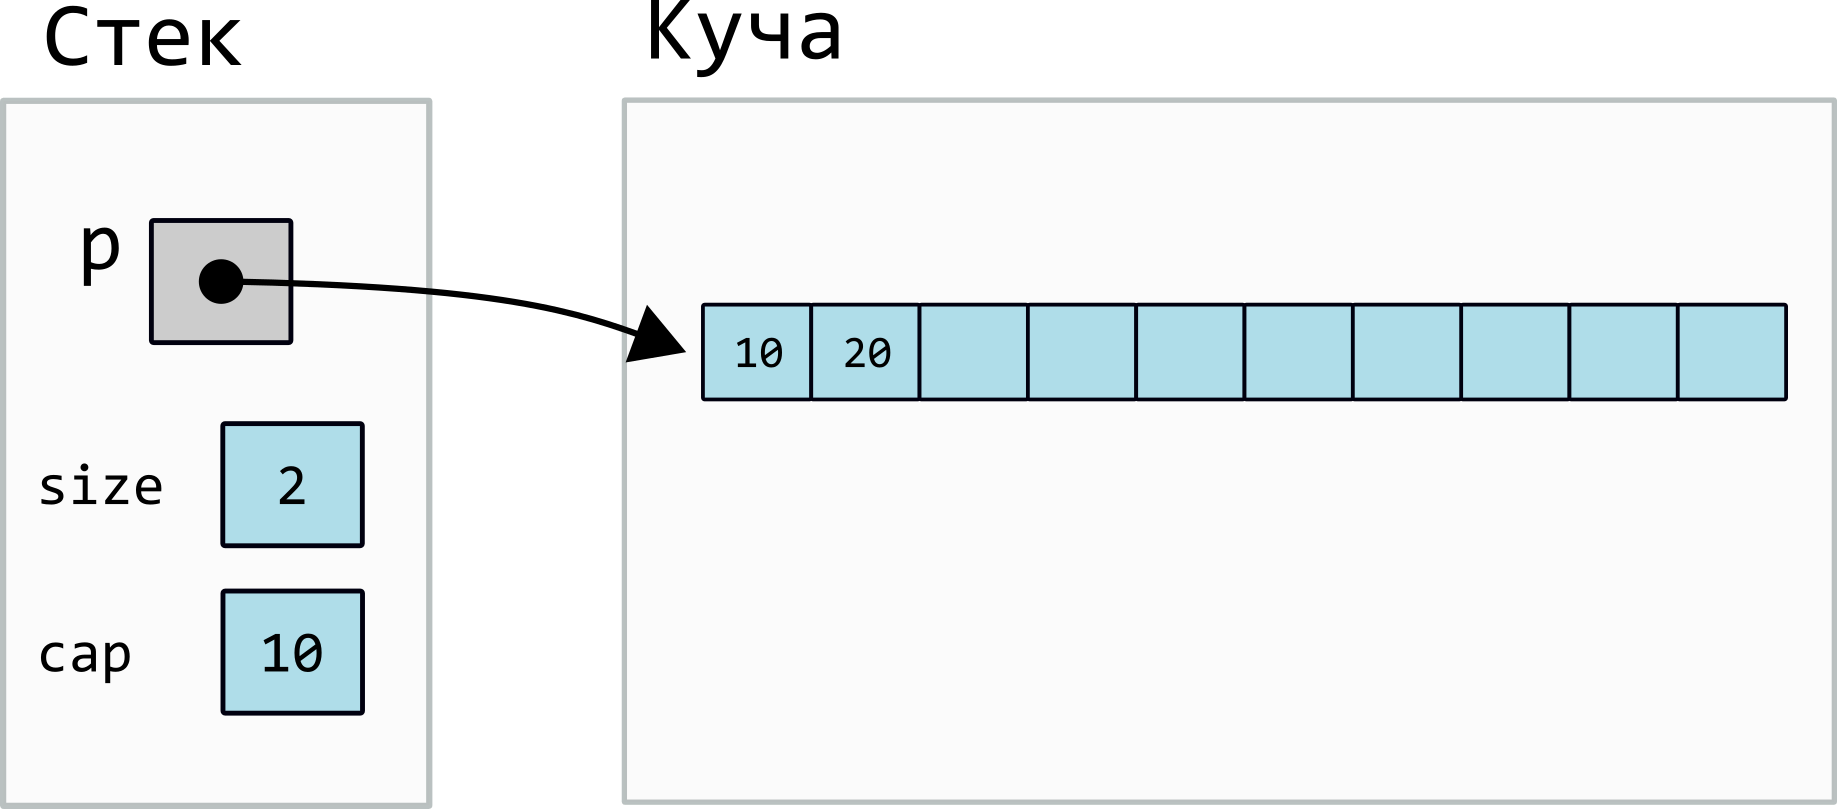
\includegraphics[scale=0.6]{images/dynamic_array/dynamic_array_cap_add_one5.png}
\end{center}
\end{frame}

\section{Динамический массив \texttt{std::vector}}

\begin{frame}[fragile]
\frametitle{Класс \texttt{std::vector}}
\begin{lstlisting}
std::vector<int> v {10, 20, 30, 40, 50};
\end{lstlisting}
\begin{center}
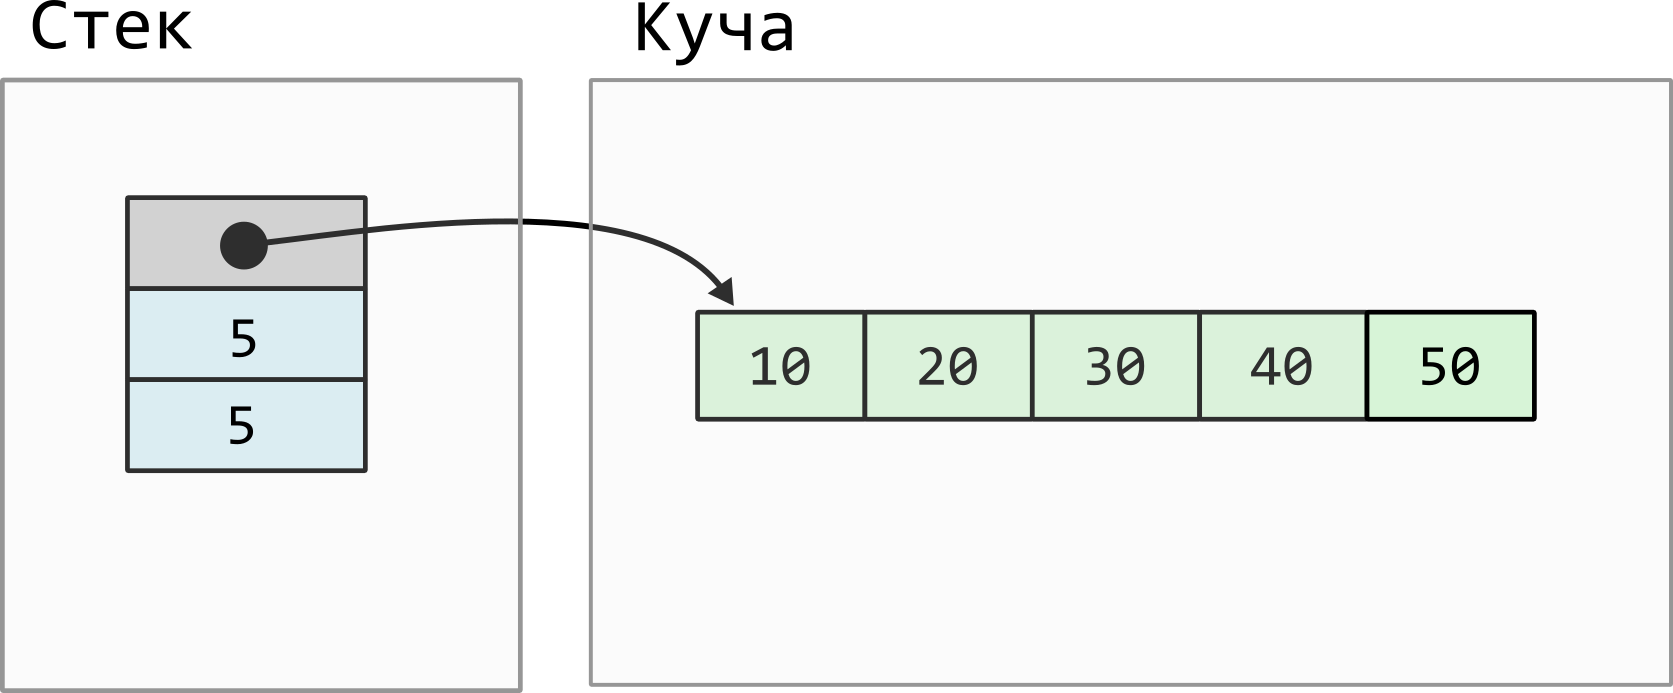
\includegraphics[scale=0.6]{images/dynamic_array/vector_implementation1.png}
\end{center}
\end{frame}


\begin{frame}[fragile]
\frametitle{Класс \texttt{std::vector}}
\begin{lstlisting}
std::vector<int> v {10, 20, 30, 40, 50};
v.push_back(60);
\end{lstlisting}
\begin{center}
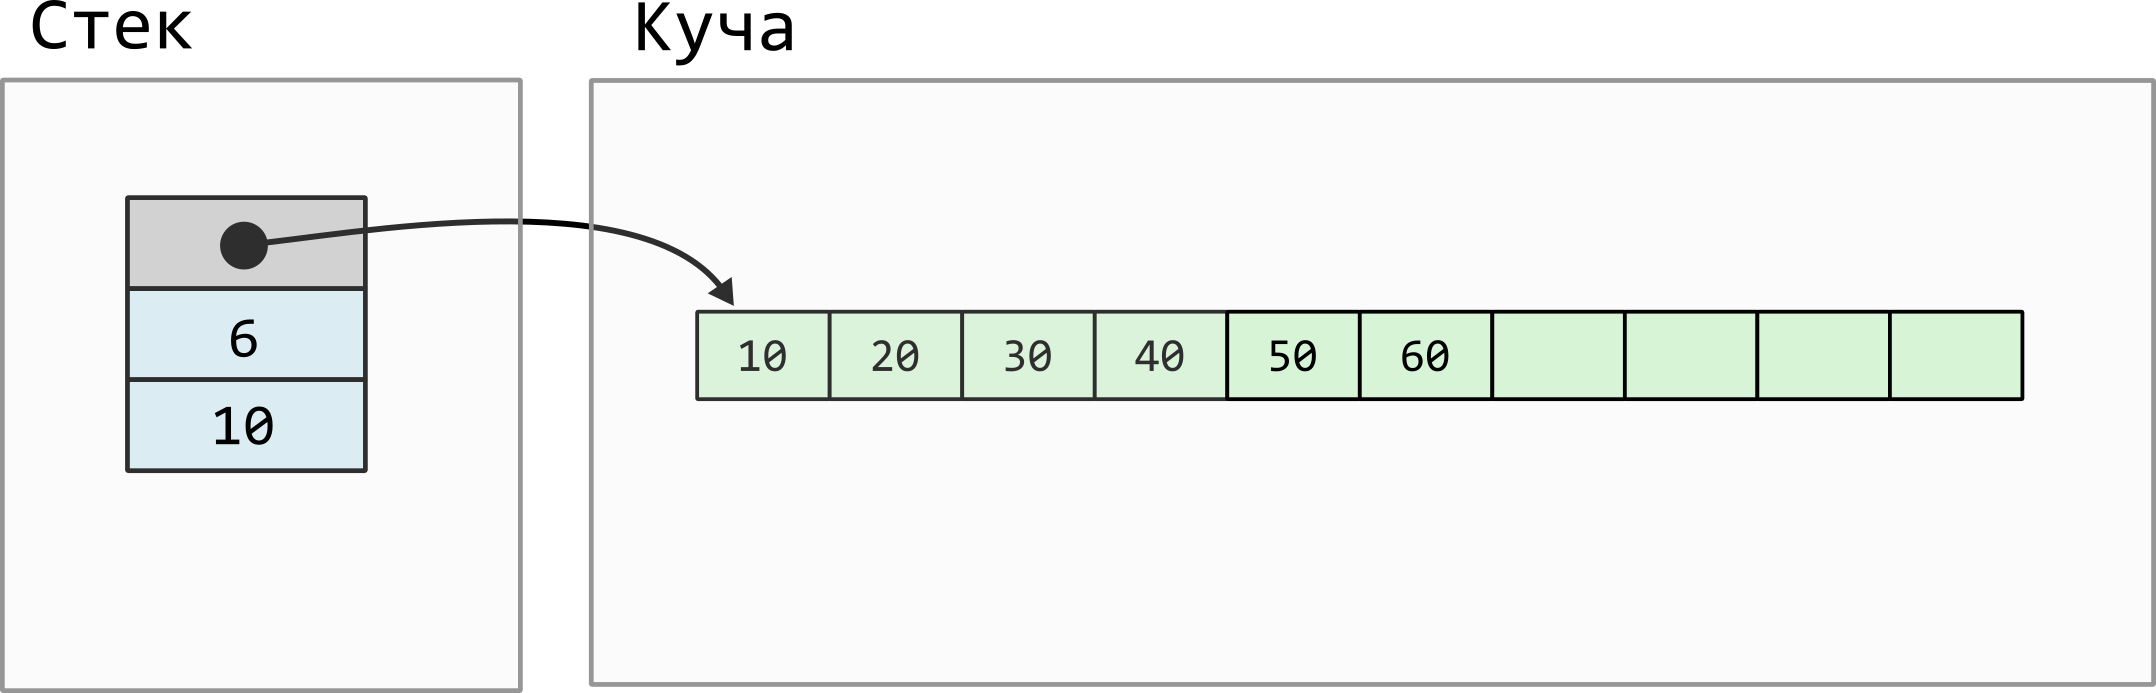
\includegraphics[scale=0.6]{images/dynamic_array/vector_implementation2.png}
\end{center}
\end{frame}


\begin{frame}[fragile]
\frametitle{Класс \texttt{std::vector}}
\begin{lstlisting}
v.push_back(70);
\end{lstlisting}
\begin{center}
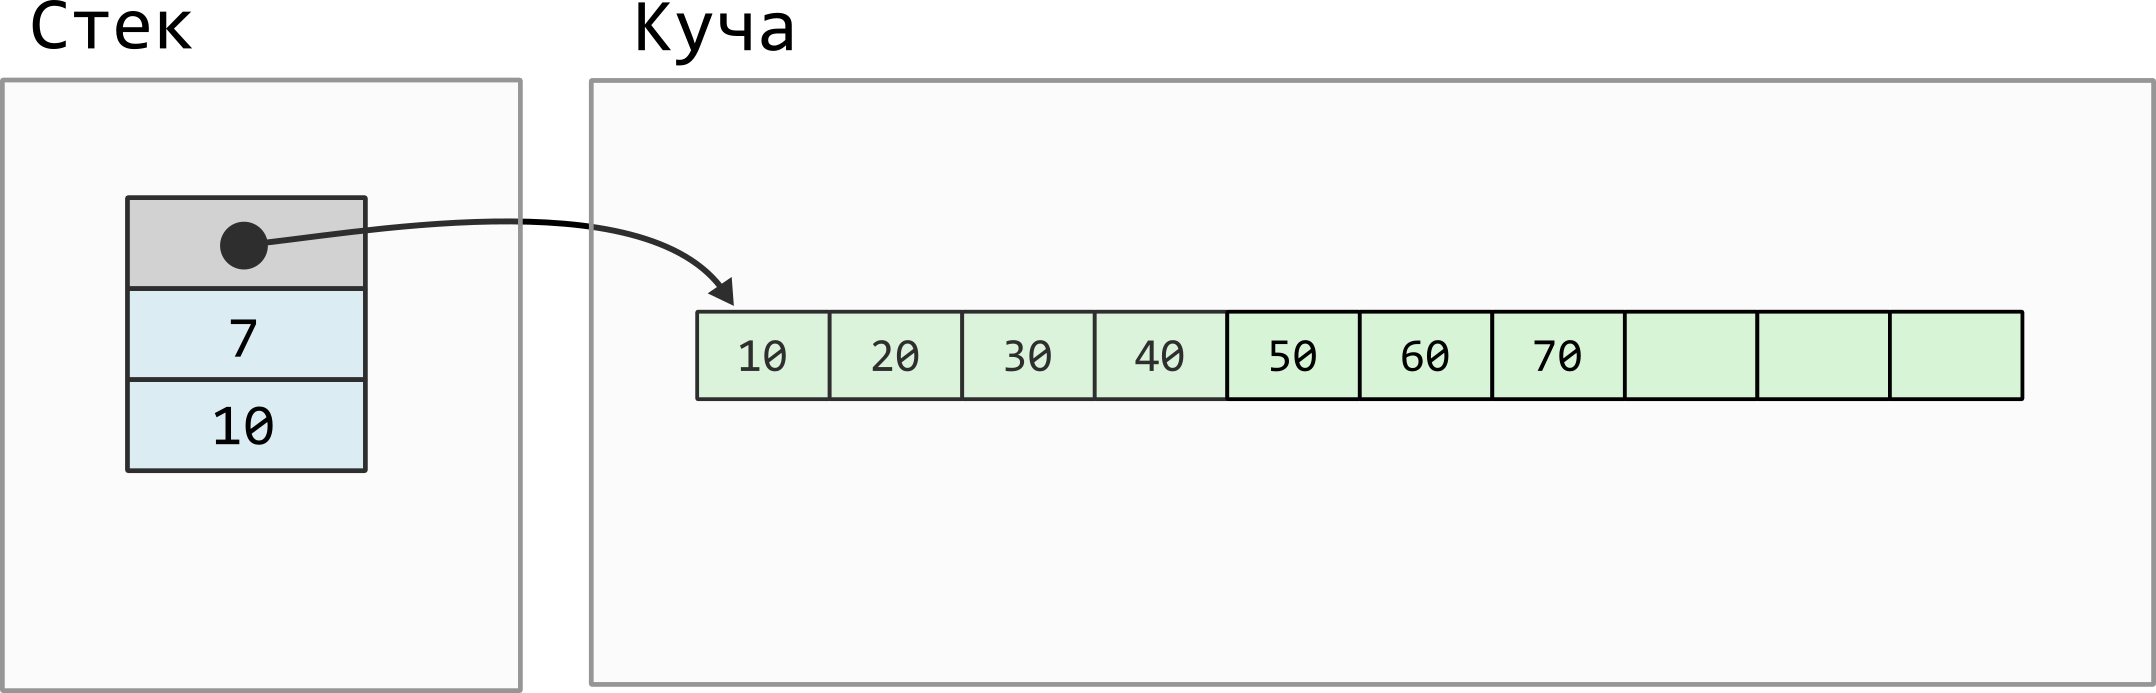
\includegraphics[scale=0.6]{images/dynamic_array/vector_implementation3.png}
\end{center}
\end{frame}


\section{Связный список}

\begin{frame}[fragile]
\frametitle{Связный список}
\begin{center}
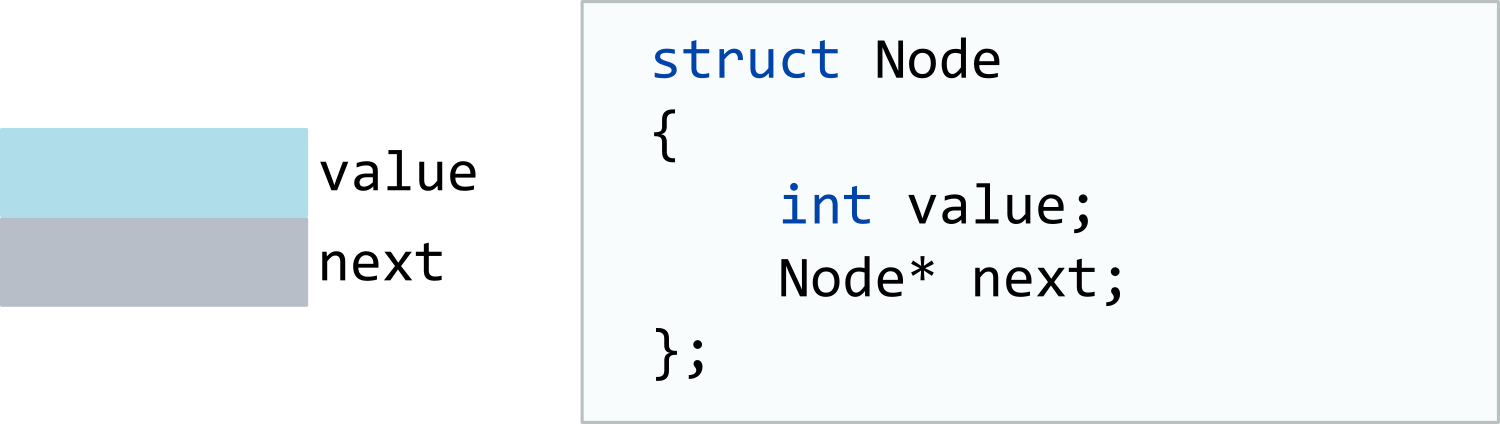
\includegraphics[scale=0.6]{images/list/structlist.png}
\end{center}
\end{frame}

\begin{frame}[fragile]
\frametitle{Связный список}
\begin{center}
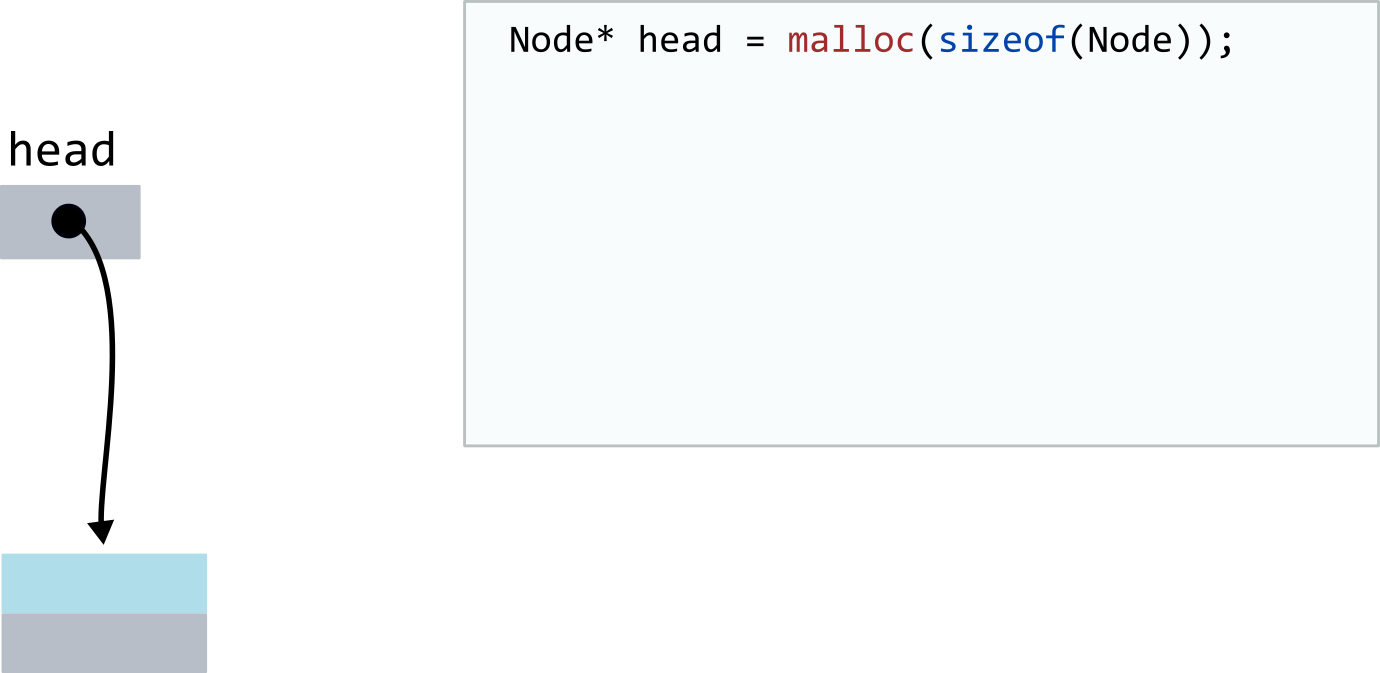
\includegraphics[scale=0.6]{images/list/codelist2.png}
\end{center}
\end{frame}


\begin{frame}[fragile]
\frametitle{Связный список}
\begin{center}
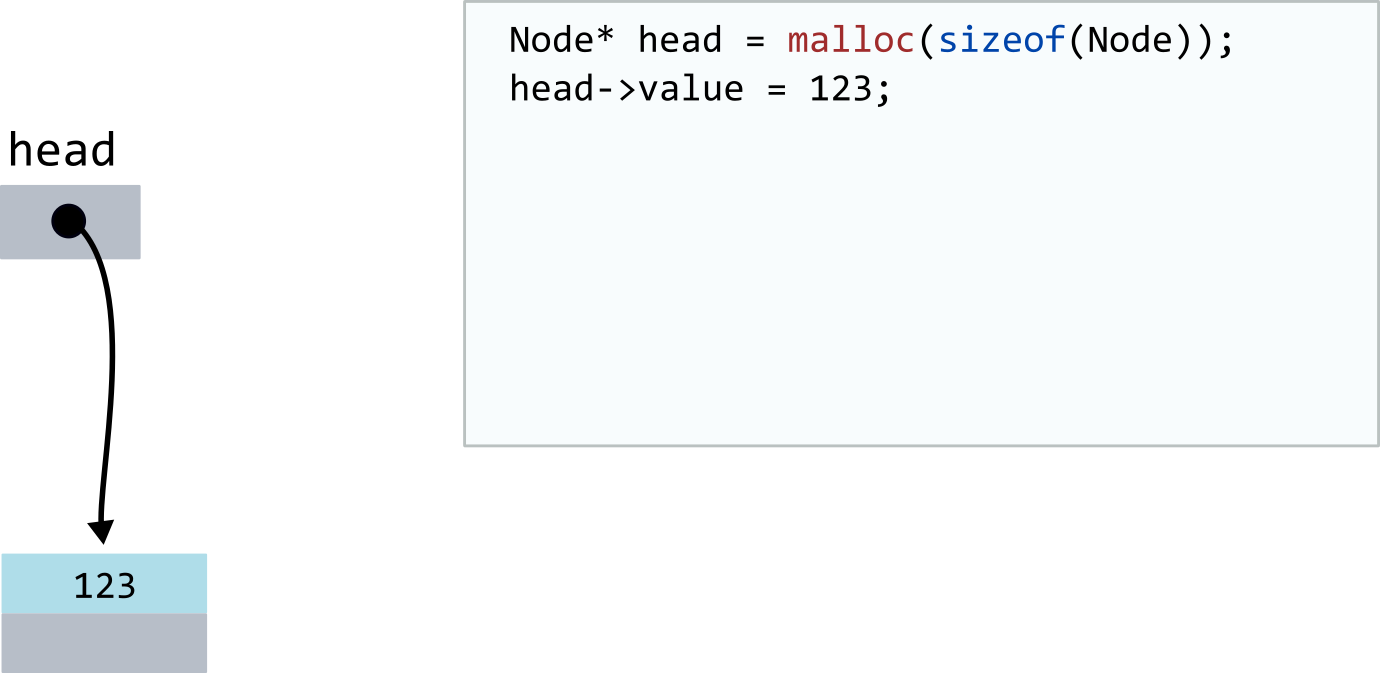
\includegraphics[scale=0.6]{images/list/codelist3.png}
\end{center}
\end{frame}


\begin{frame}[fragile]
\frametitle{Связный список}
\begin{center}
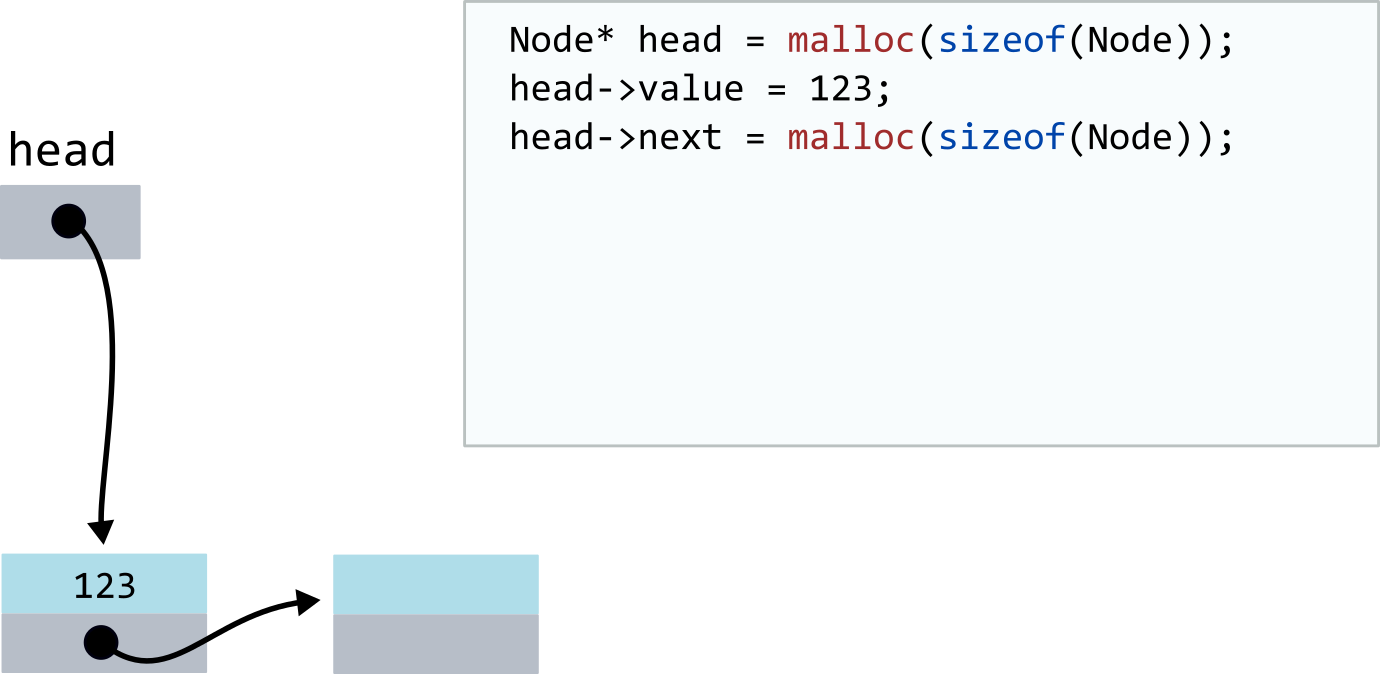
\includegraphics[scale=0.6]{images/list/codelist4.png}
\end{center}
\end{frame}


\begin{frame}[fragile]
\frametitle{Связный список}
\begin{center}
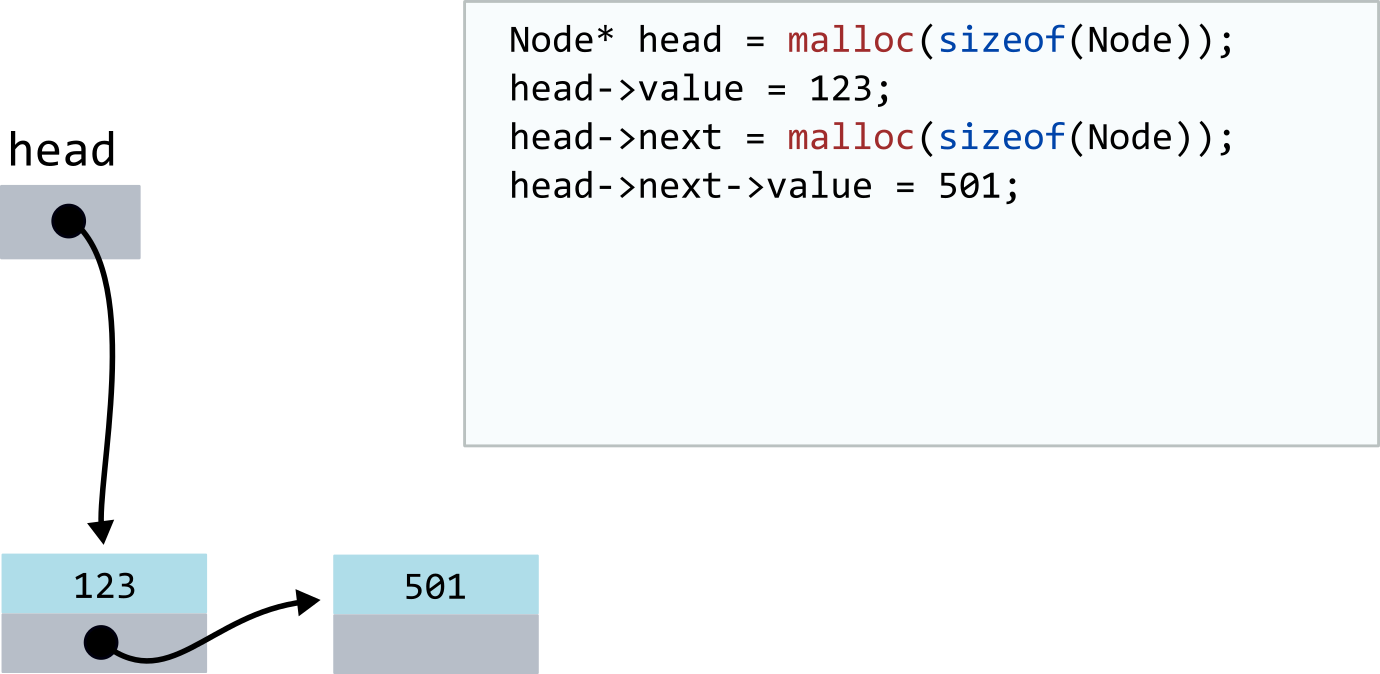
\includegraphics[scale=0.6]{images/list/codelist5.png}
\end{center}
\end{frame}


\begin{frame}[fragile]
\frametitle{Связный список}
\begin{center}
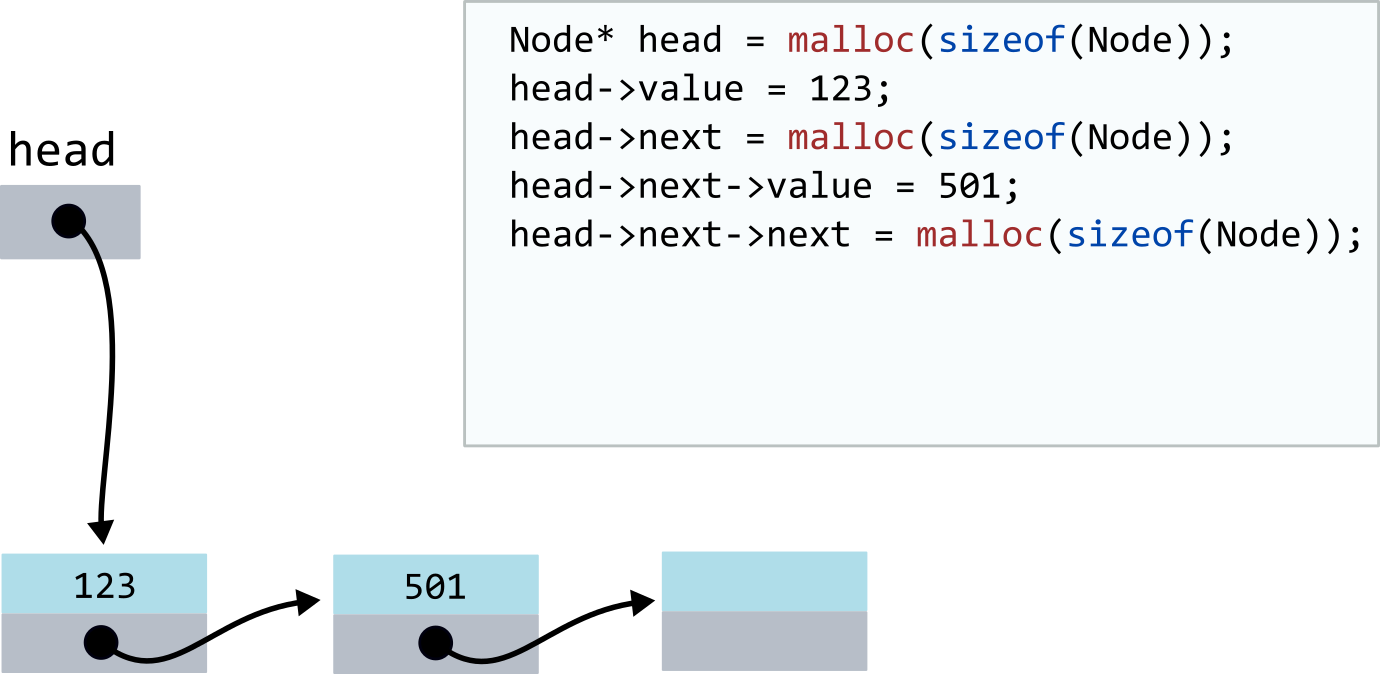
\includegraphics[scale=0.6]{images/list/codelist6.png}
\end{center}
\end{frame}

\begin{frame}[fragile]
\frametitle{Связный список}
\begin{center}
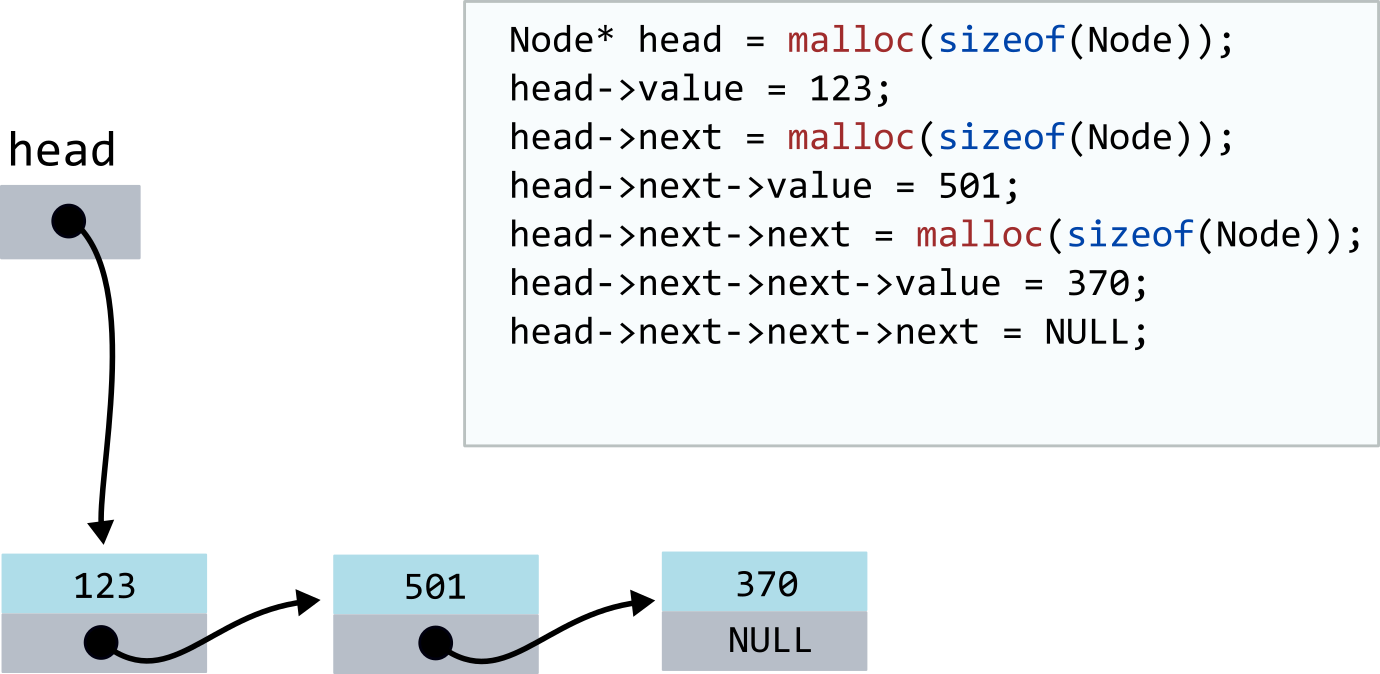
\includegraphics[scale=0.6]{images/list/codelist7.png}
\end{center}
\end{frame}

\section{Добавление элемента в связный список}

\begin{frame}[fragile]
\frametitle{Добавление элемента в связный список}
\begin{center}
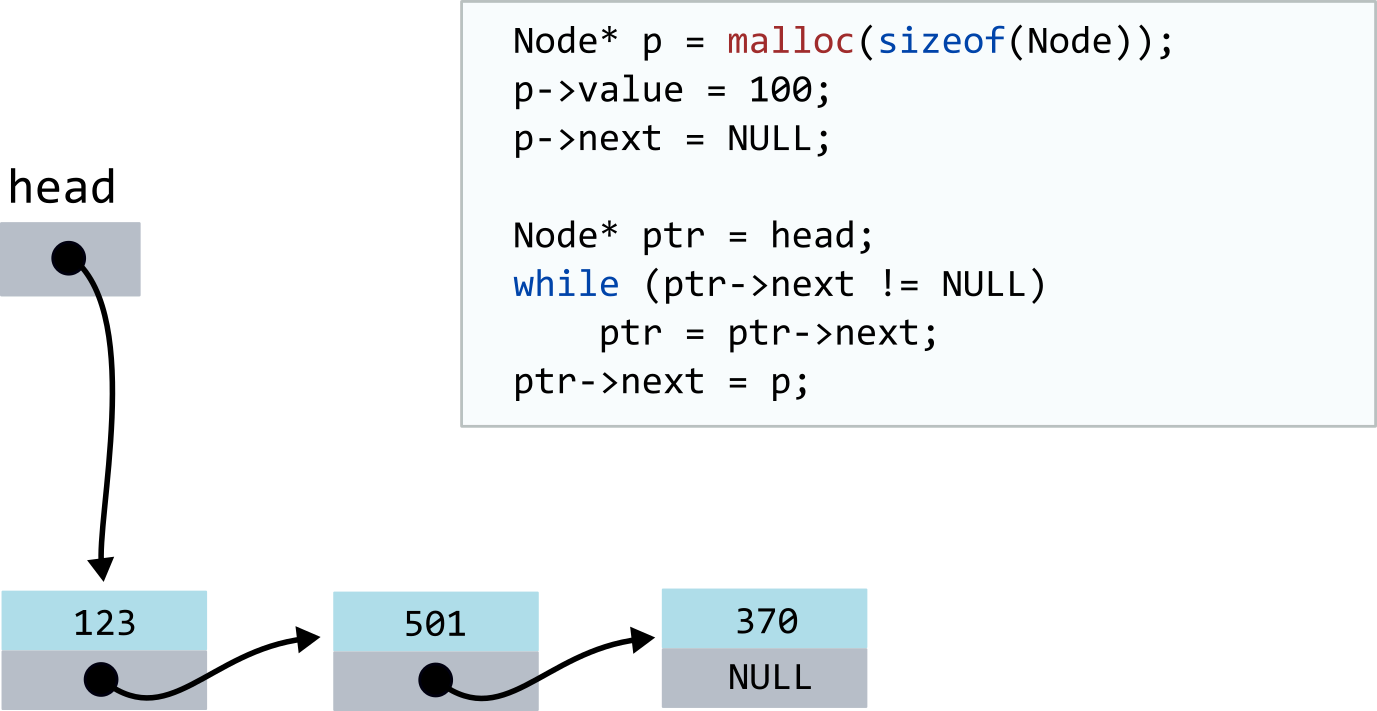
\includegraphics[scale=0.6]{images/list/codelistf_insert1.png}
\end{center}
\end{frame}


\begin{frame}[fragile]
\frametitle{Добавление элемента в связный список}
\begin{center}
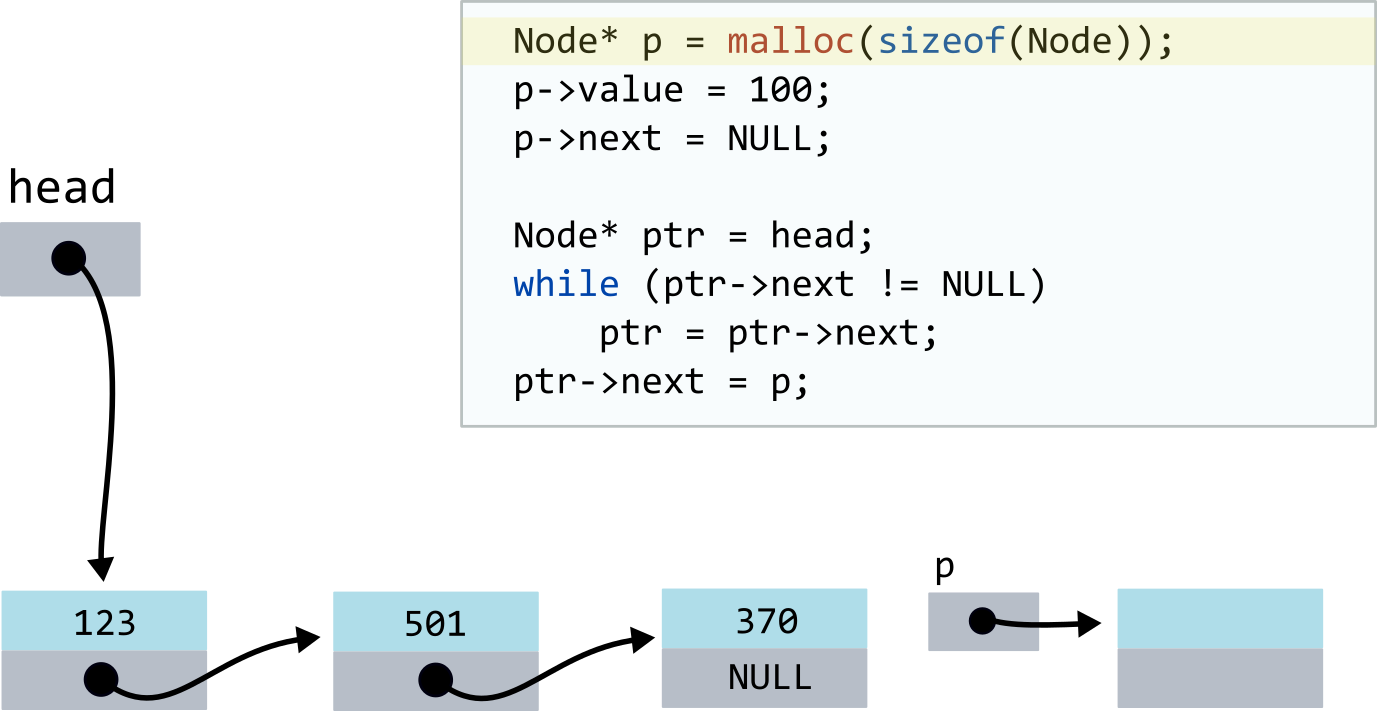
\includegraphics[scale=0.6]{images/list/codelistf_insert2.png}
\end{center}
\end{frame}


\begin{frame}[fragile]
\frametitle{Добавление элемента в связный список}
\begin{center}
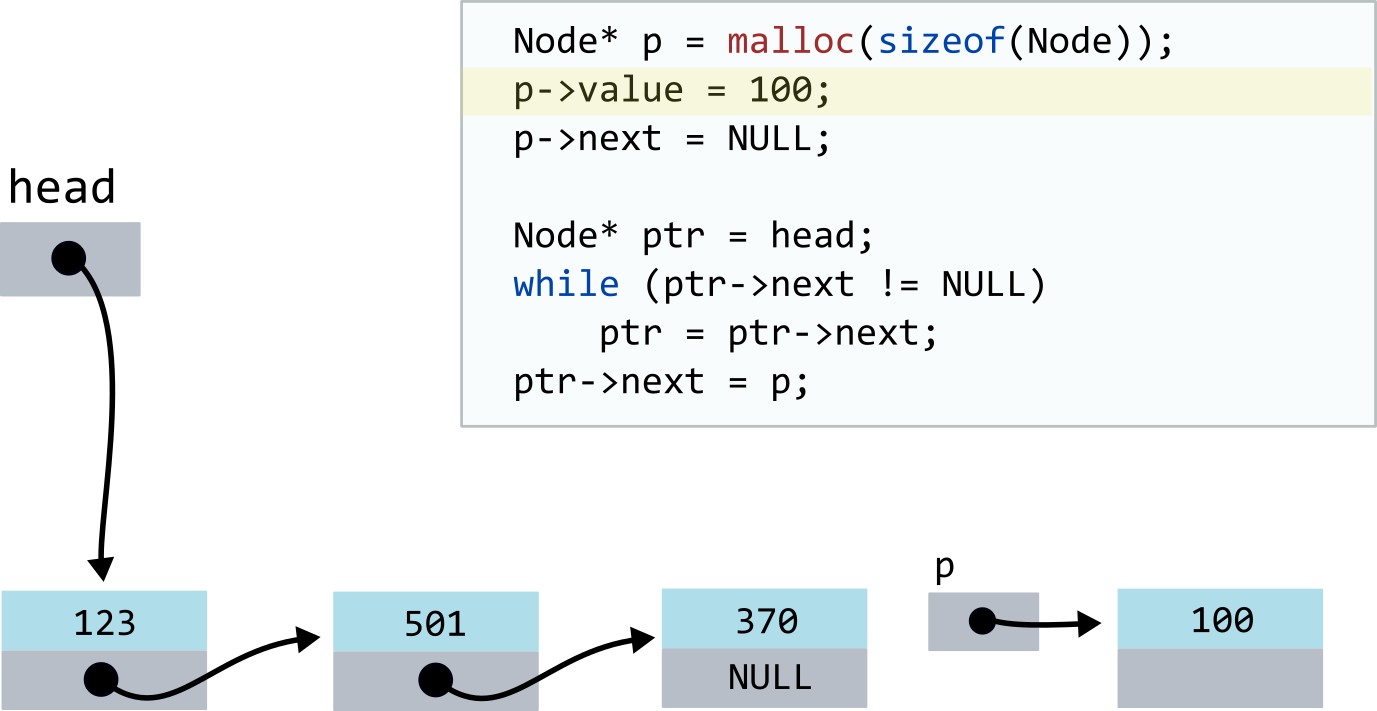
\includegraphics[scale=0.6]{images/list/codelistf_insert3.png}
\end{center}
\end{frame}

\begin{frame}[fragile]
\frametitle{Добавление элемента в связный список}
\begin{center}
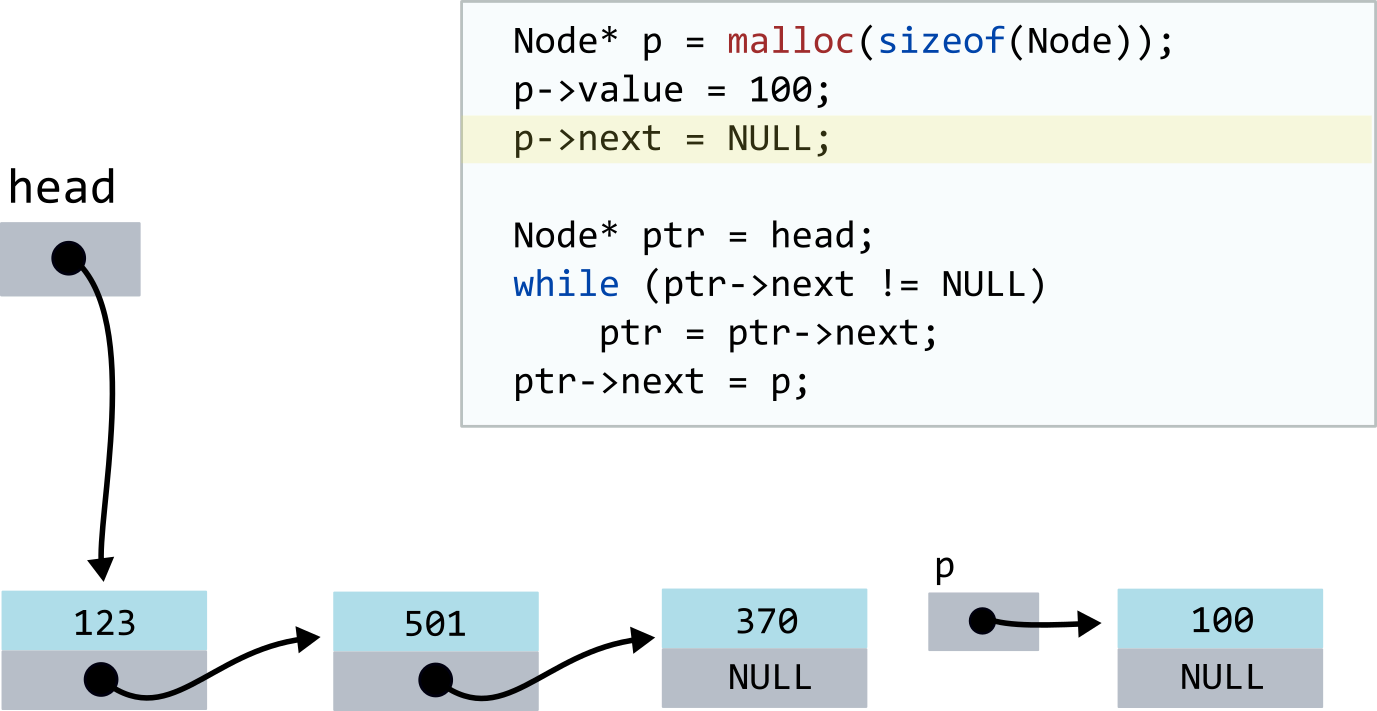
\includegraphics[scale=0.6]{images/list/codelistf_insert4.png}
\end{center}
\end{frame}


\begin{frame}[fragile]
\frametitle{Добавление элемента в связный список}
\begin{center}
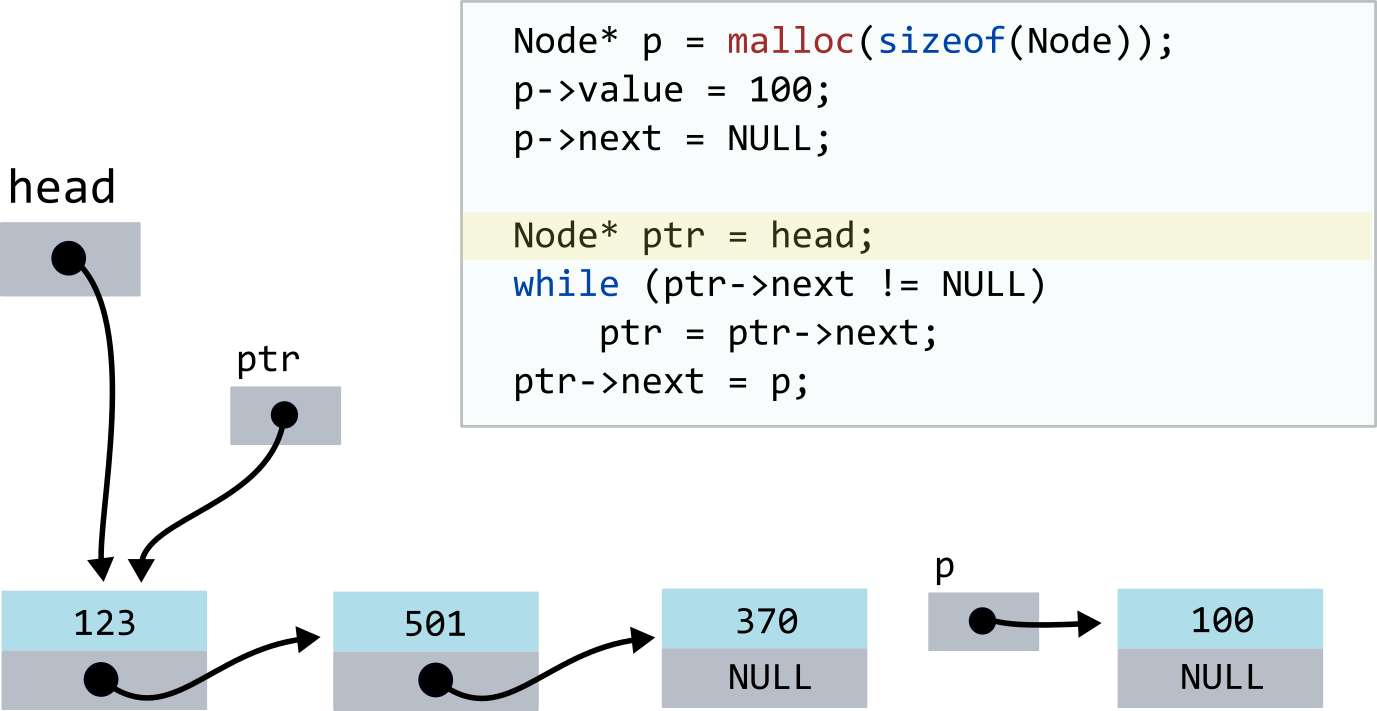
\includegraphics[scale=0.6]{images/list/codelistf_insert5.png}
\end{center}
\end{frame}


\begin{frame}[fragile]
\frametitle{Добавление элемента в связный список}
\begin{center}
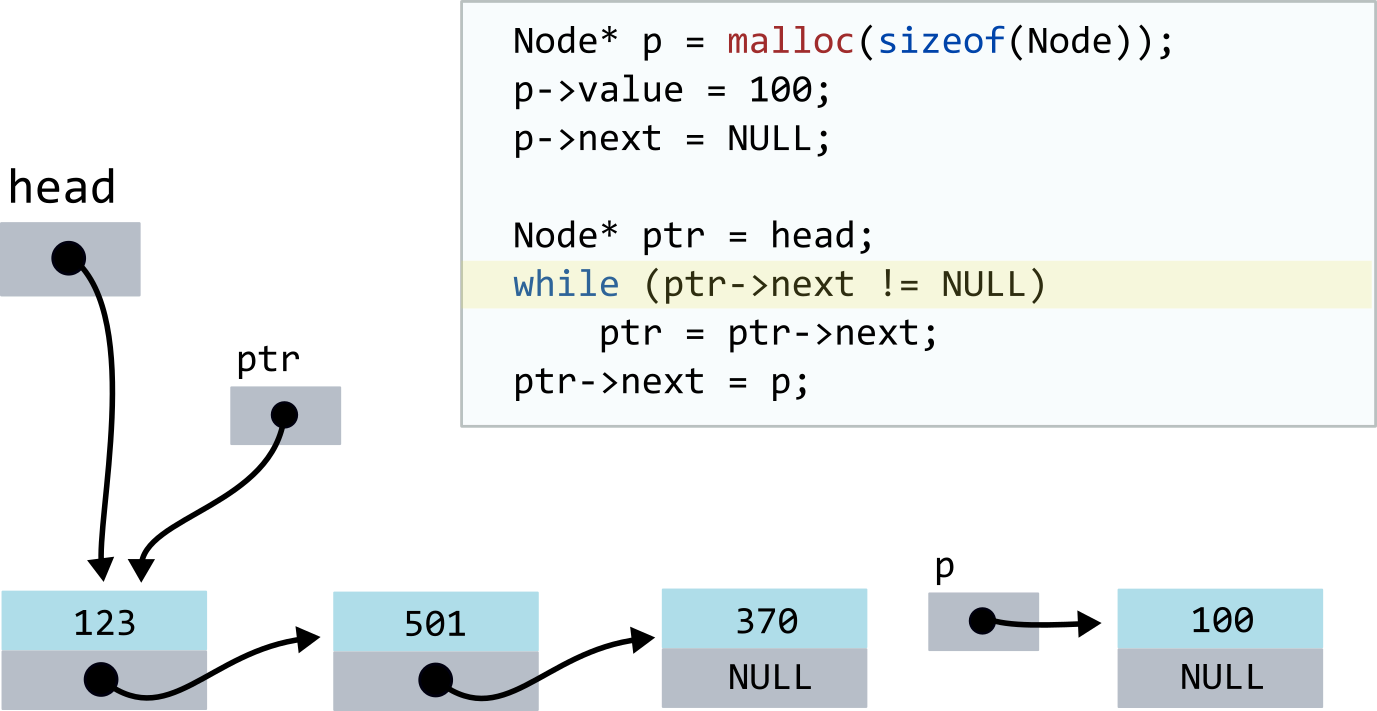
\includegraphics[scale=0.6]{images/list/codelistf_insert6.png}
\end{center}
\end{frame}


\begin{frame}[fragile]
\frametitle{Добавление элемента в связный список}
\begin{center}
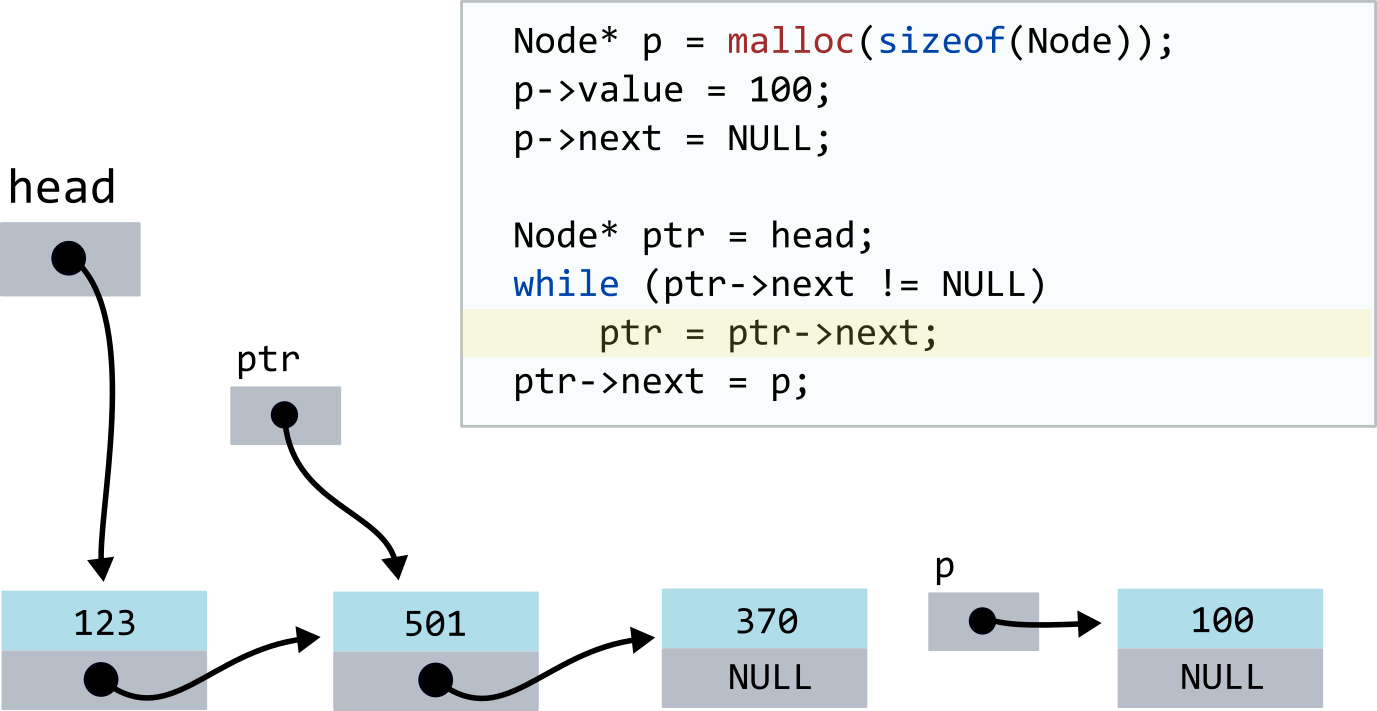
\includegraphics[scale=0.6]{images/list/codelistf_insert7.png}
\end{center}
\end{frame}


\begin{frame}[fragile]
\frametitle{Добавление элемента в связный список}
\begin{center}
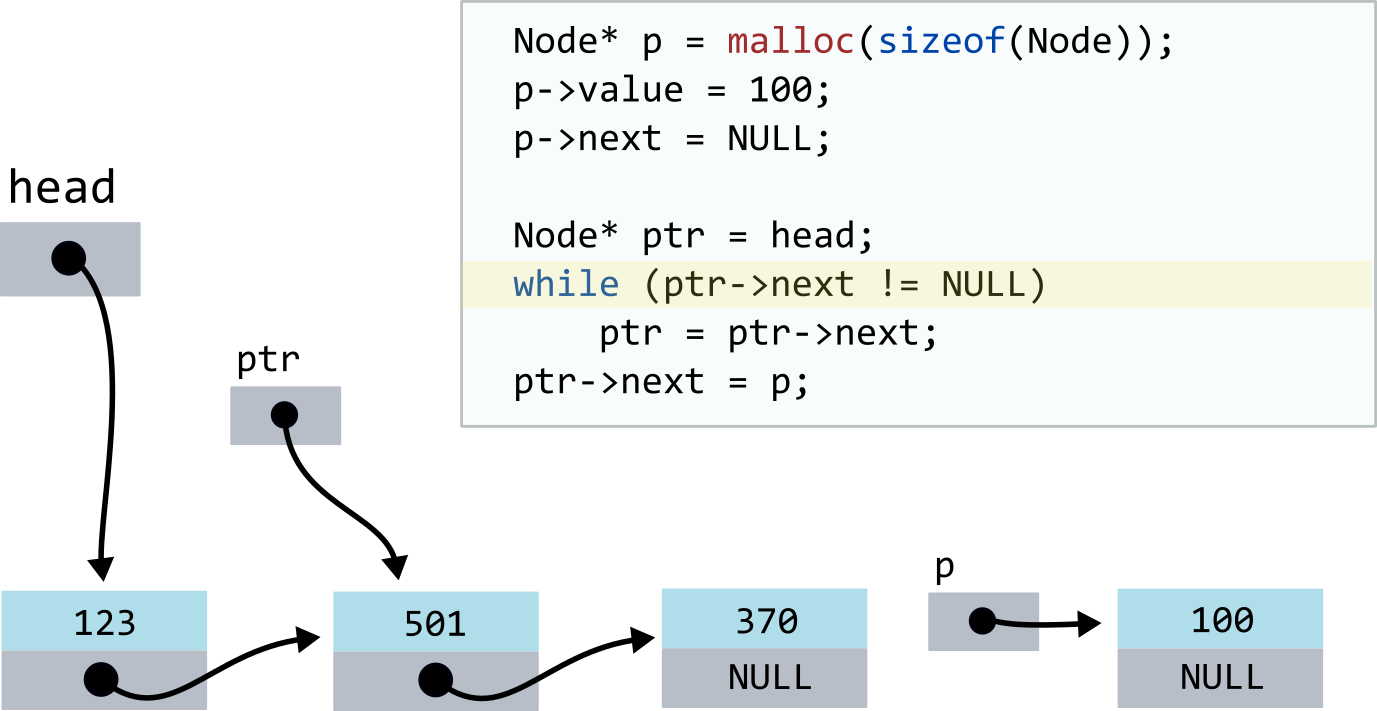
\includegraphics[scale=0.6]{images/list/codelistf_insert8.png}
\end{center}
\end{frame}


\begin{frame}[fragile]
\frametitle{Добавление элемента в связный список}
\begin{center}
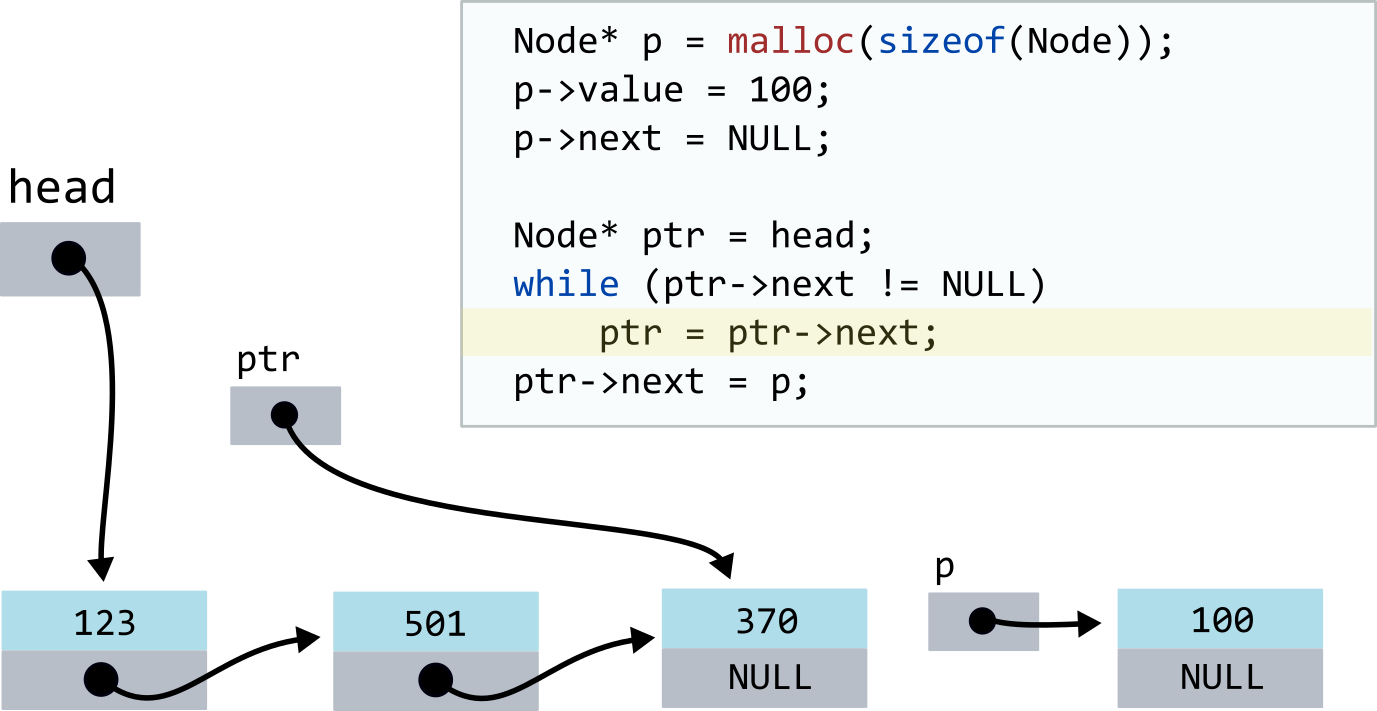
\includegraphics[scale=0.6]{images/list/codelistf_insert9.png}
\end{center}
\end{frame}


\begin{frame}[fragile]
\frametitle{Добавление элемента в связный список}
\begin{center}
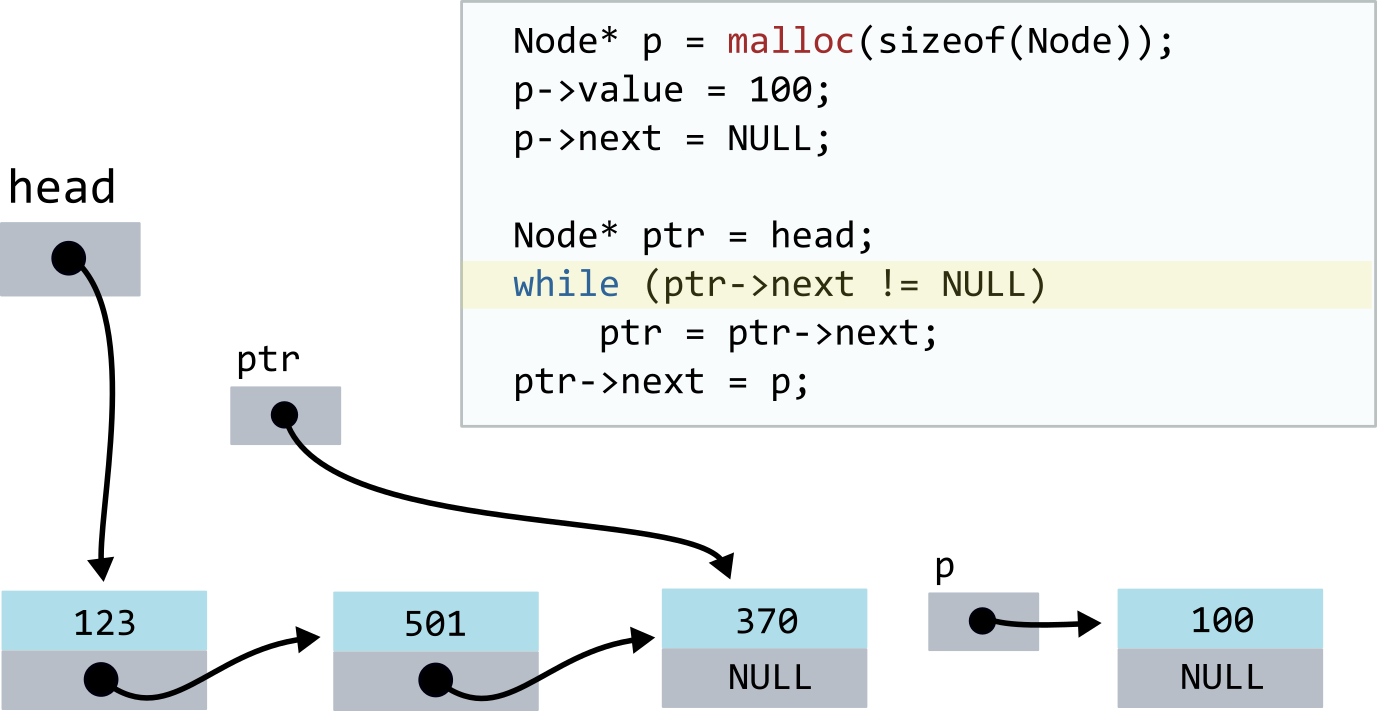
\includegraphics[scale=0.6]{images/list/codelistf_insert10.png}
\end{center}
\end{frame}

\begin{frame}[fragile]
\frametitle{Добавление элемента в связный список}
\begin{center}
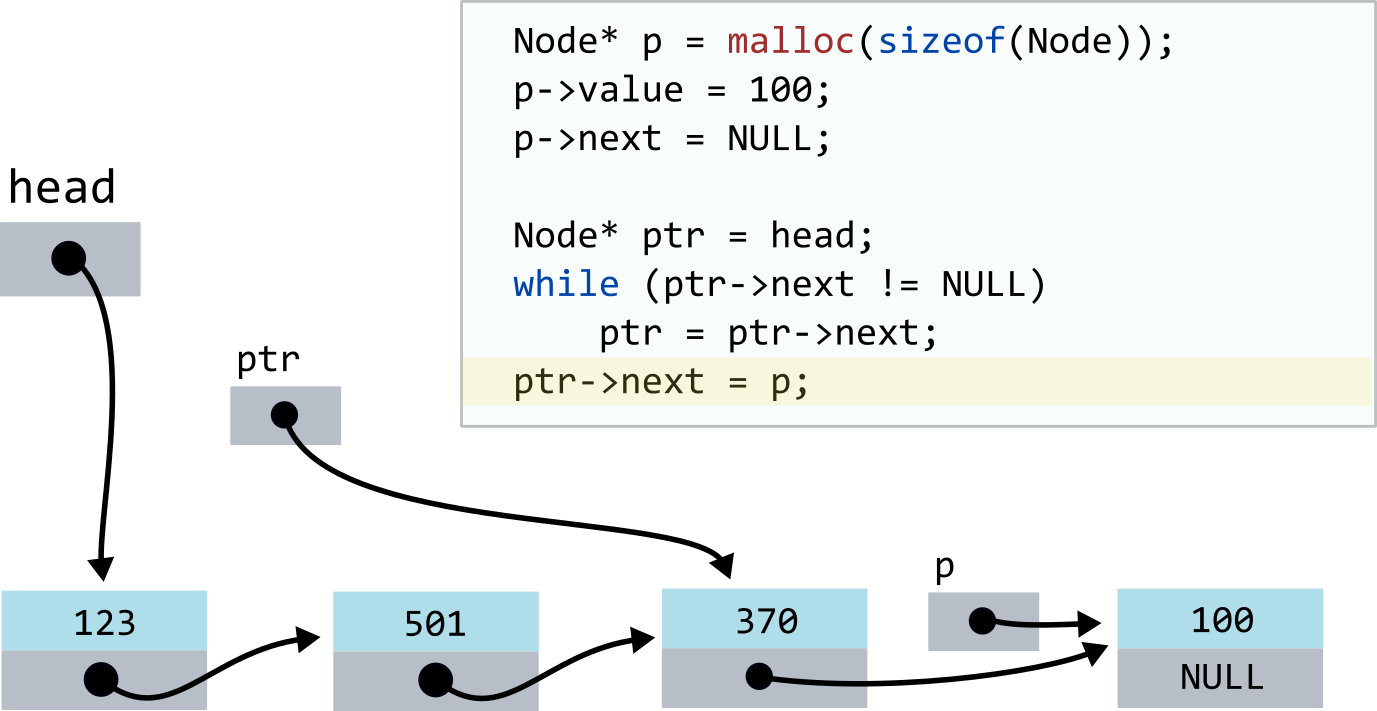
\includegraphics[scale=0.6]{images/list/codelistf_insert11.png}
\end{center}
\end{frame}


\begin{frame}[fragile]
\frametitle{Добавление элемента в связный список}
\begin{center}
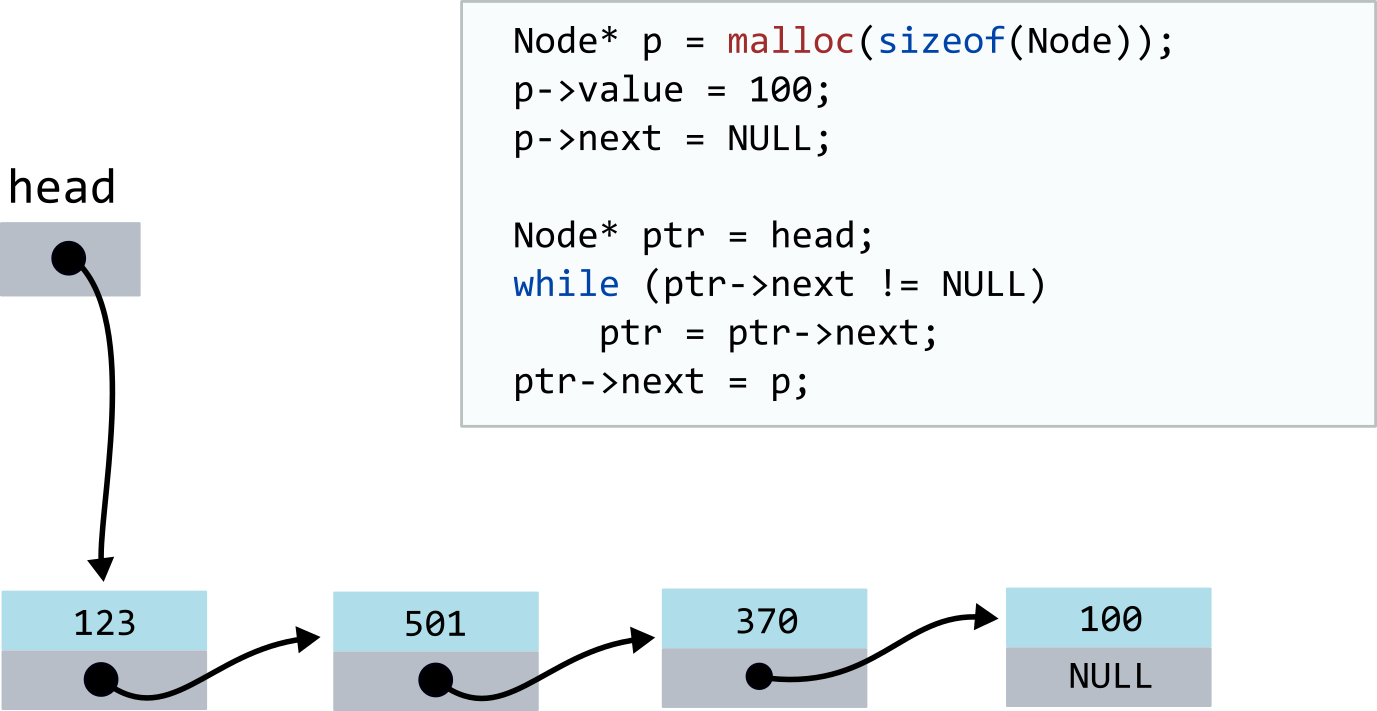
\includegraphics[scale=0.6]{images/list/codelistf_insert12.png}
\end{center}
\end{frame}


\section{Двусвязный список}

\begin{frame}[fragile]
\frametitle{Двусвязный список}
\begin{center}
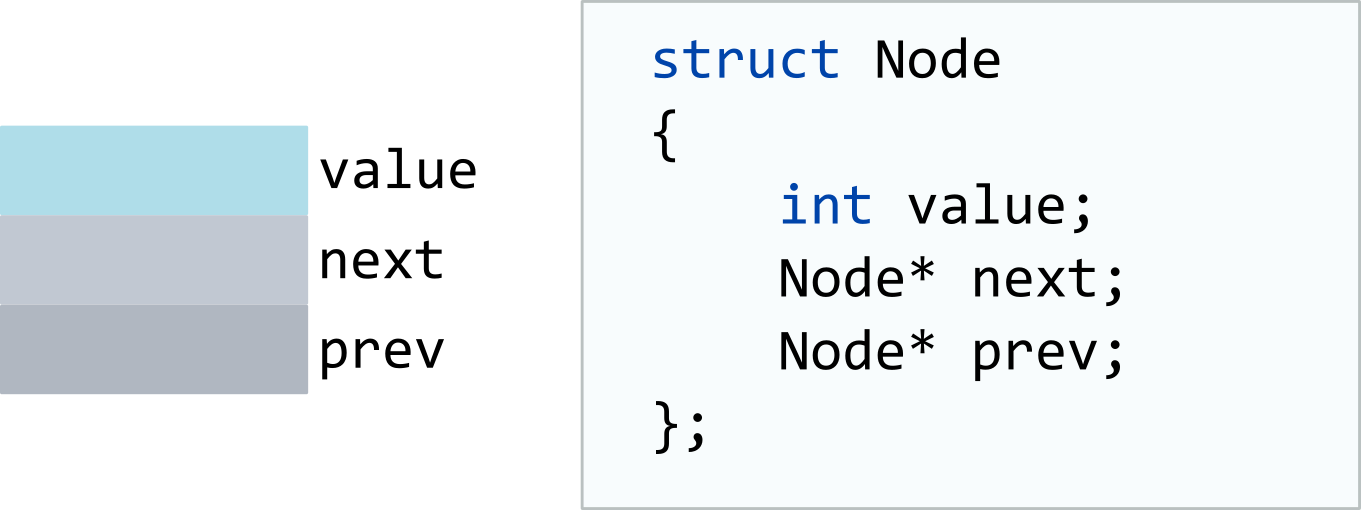
\includegraphics[scale=0.6]{images/list/doublylist_definition.png}
\end{center}
\end{frame}

\begin{frame}[fragile]
\frametitle{Двусвязный список}
\begin{center}
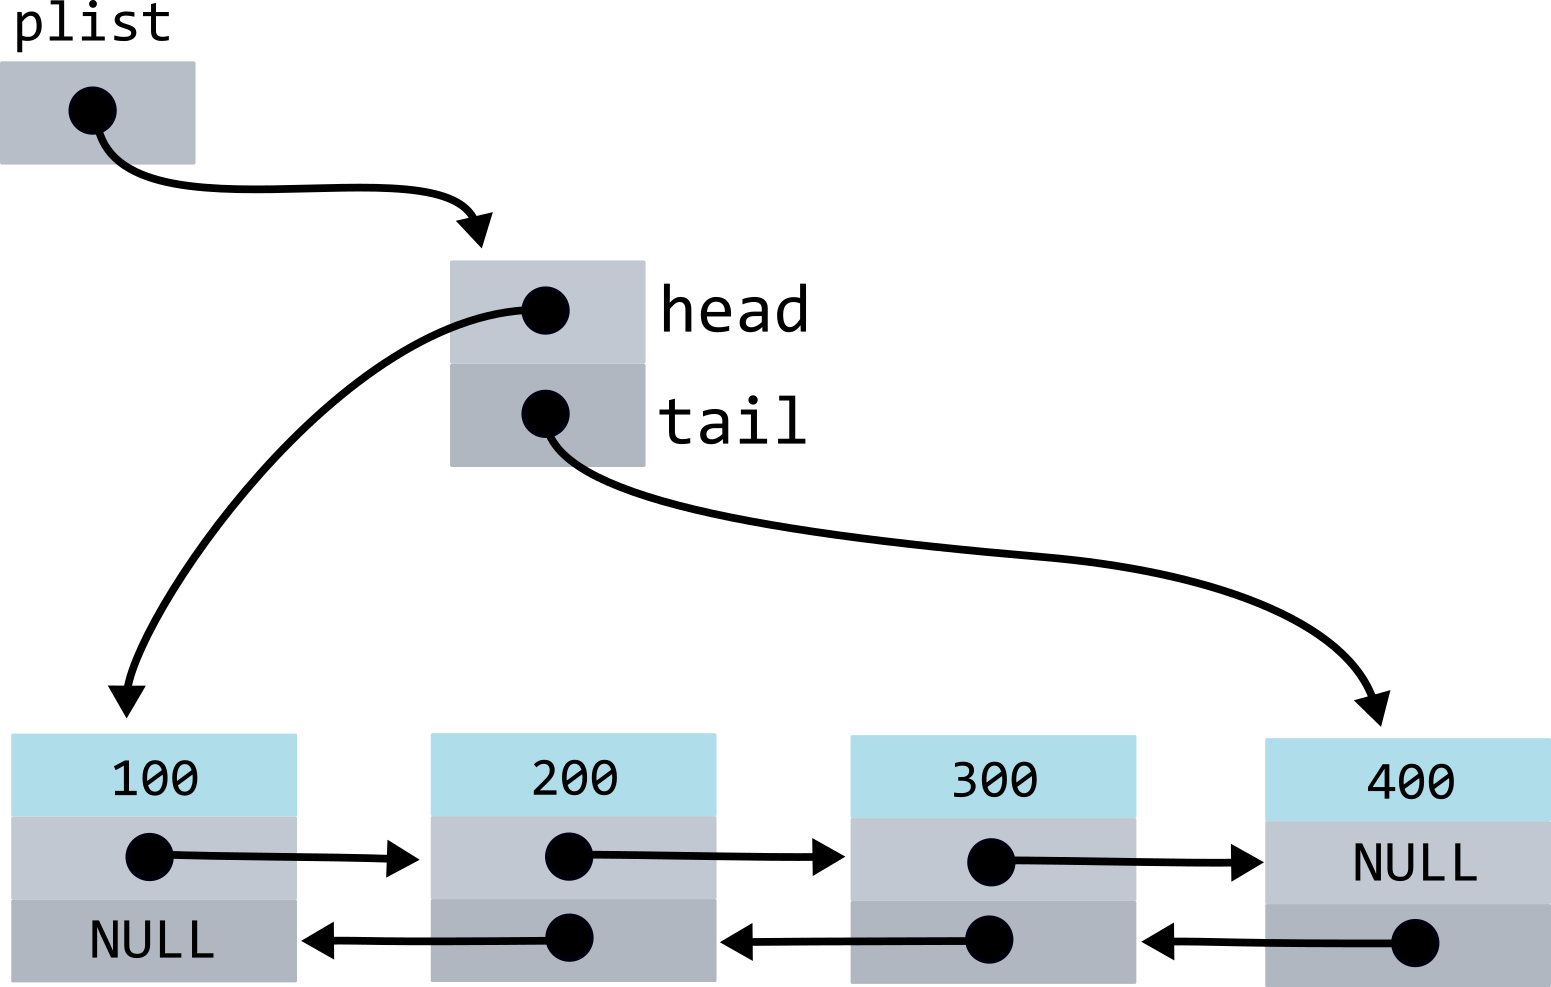
\includegraphics[scale=0.6]{images/list/doublylist_overview.png}
\end{center}
\end{frame}

\section{Связные списки в стандартной библиотеке C++. \texttt{std::list} и \texttt{std::forward\_list}}

\begin{frame}[fragile]
\frametitle{\texttt{std::list} и \texttt{std::forward\_list}}
\begin{itemize}
\item \texttt{std::forward\_list} - это односвязный список
\begin{lstlisting}
std::forward_list a {100, 200, 300, 400};
a.push_front(500);
\end{lstlisting}

\item \texttt{std::list} - это двусвязный список
\begin{lstlisting}
std::list a {100, 200, 300, 400};
a.push_front(500);
a.push_back(500);
\end{lstlisting}
\end{itemize}
\end{frame}


\section{Бинарное дерево}

\begin{frame}[fragile]
\frametitle{Бинарное дерево}
\begin{center}
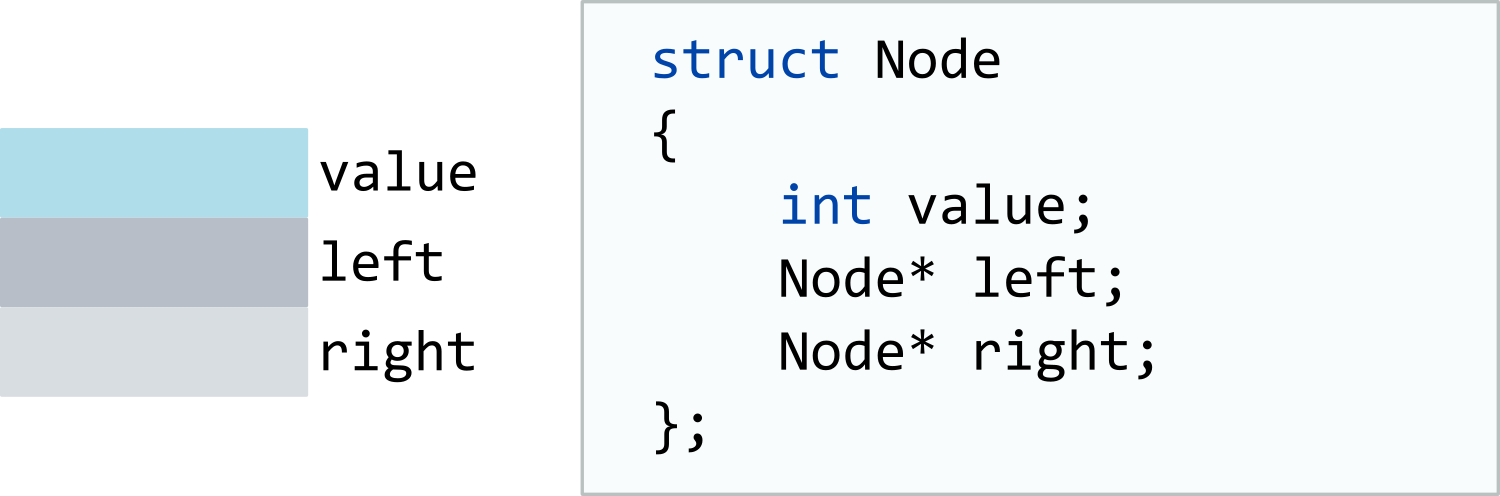
\includegraphics[scale=0.8]{images/tree/structtree.png}
\end{center}
\end{frame}


\begin{frame}[fragile]
\frametitle{Бинарное дерево}
\begin{center}
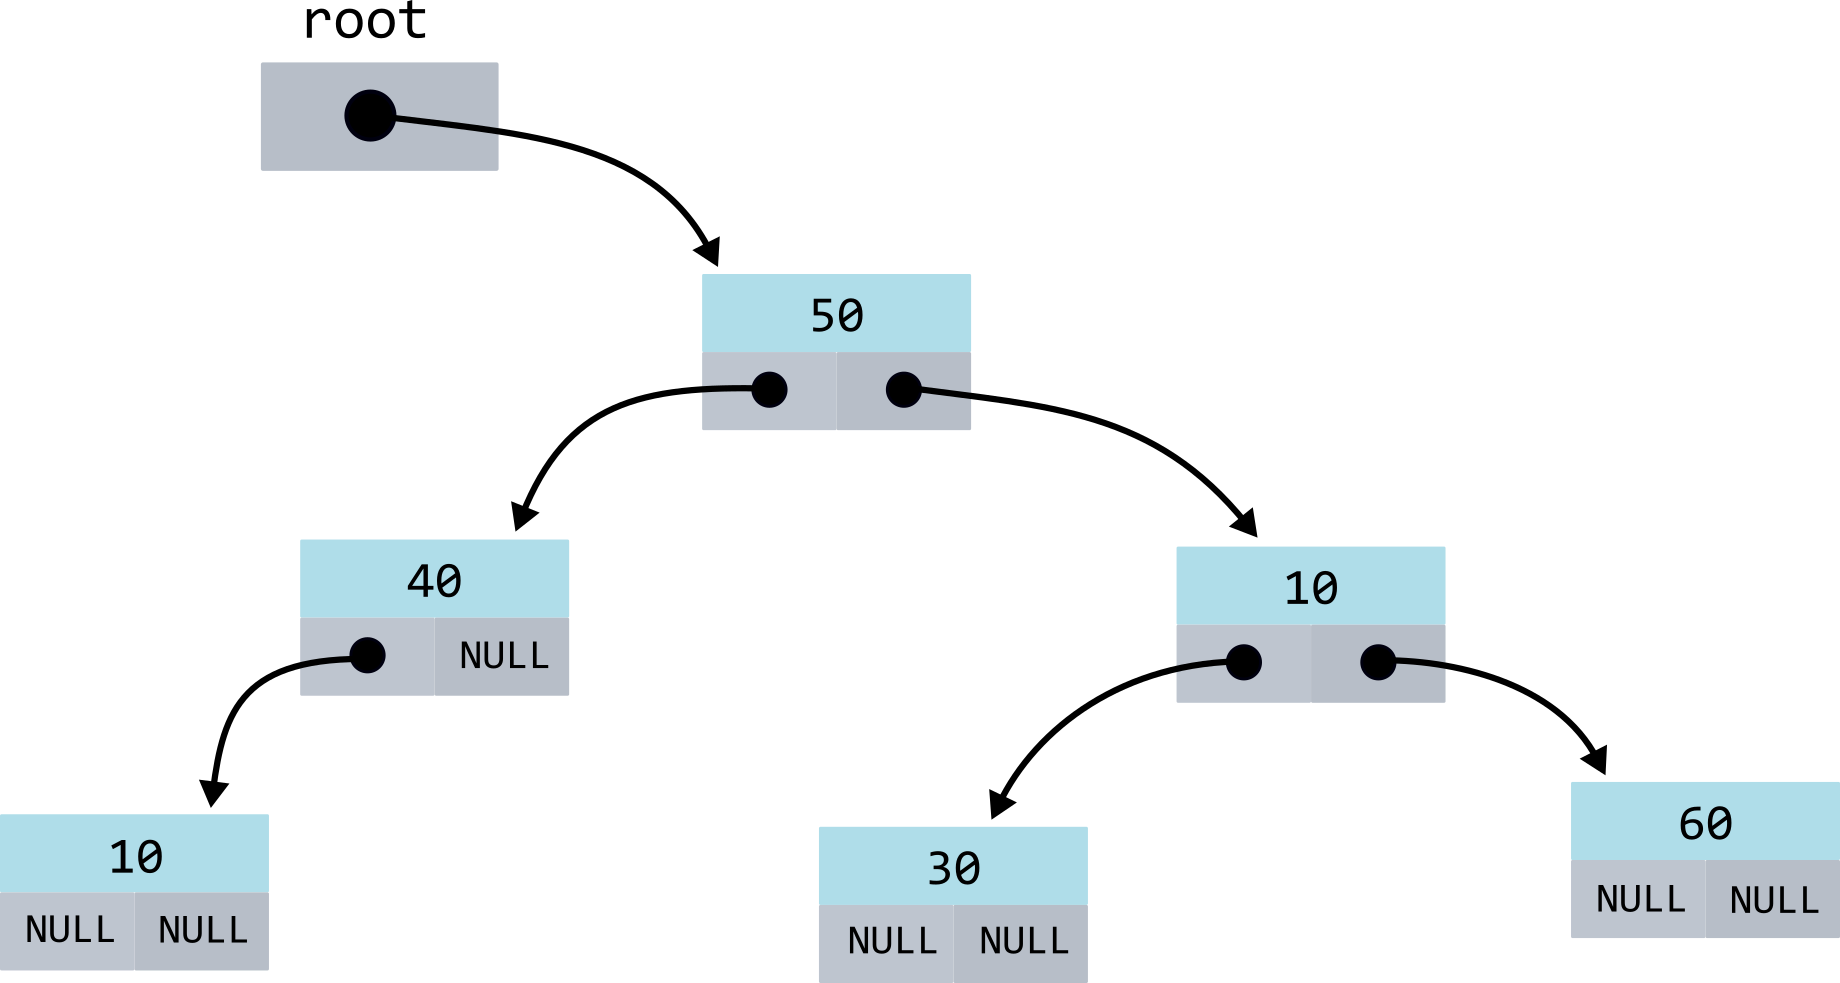
\includegraphics[scale=0.6]{images/tree/bt.png}
\end{center}
\end{frame}

\begin{frame}[fragile]
\frametitle{Бинарное дерево поиска}
\begin{center}
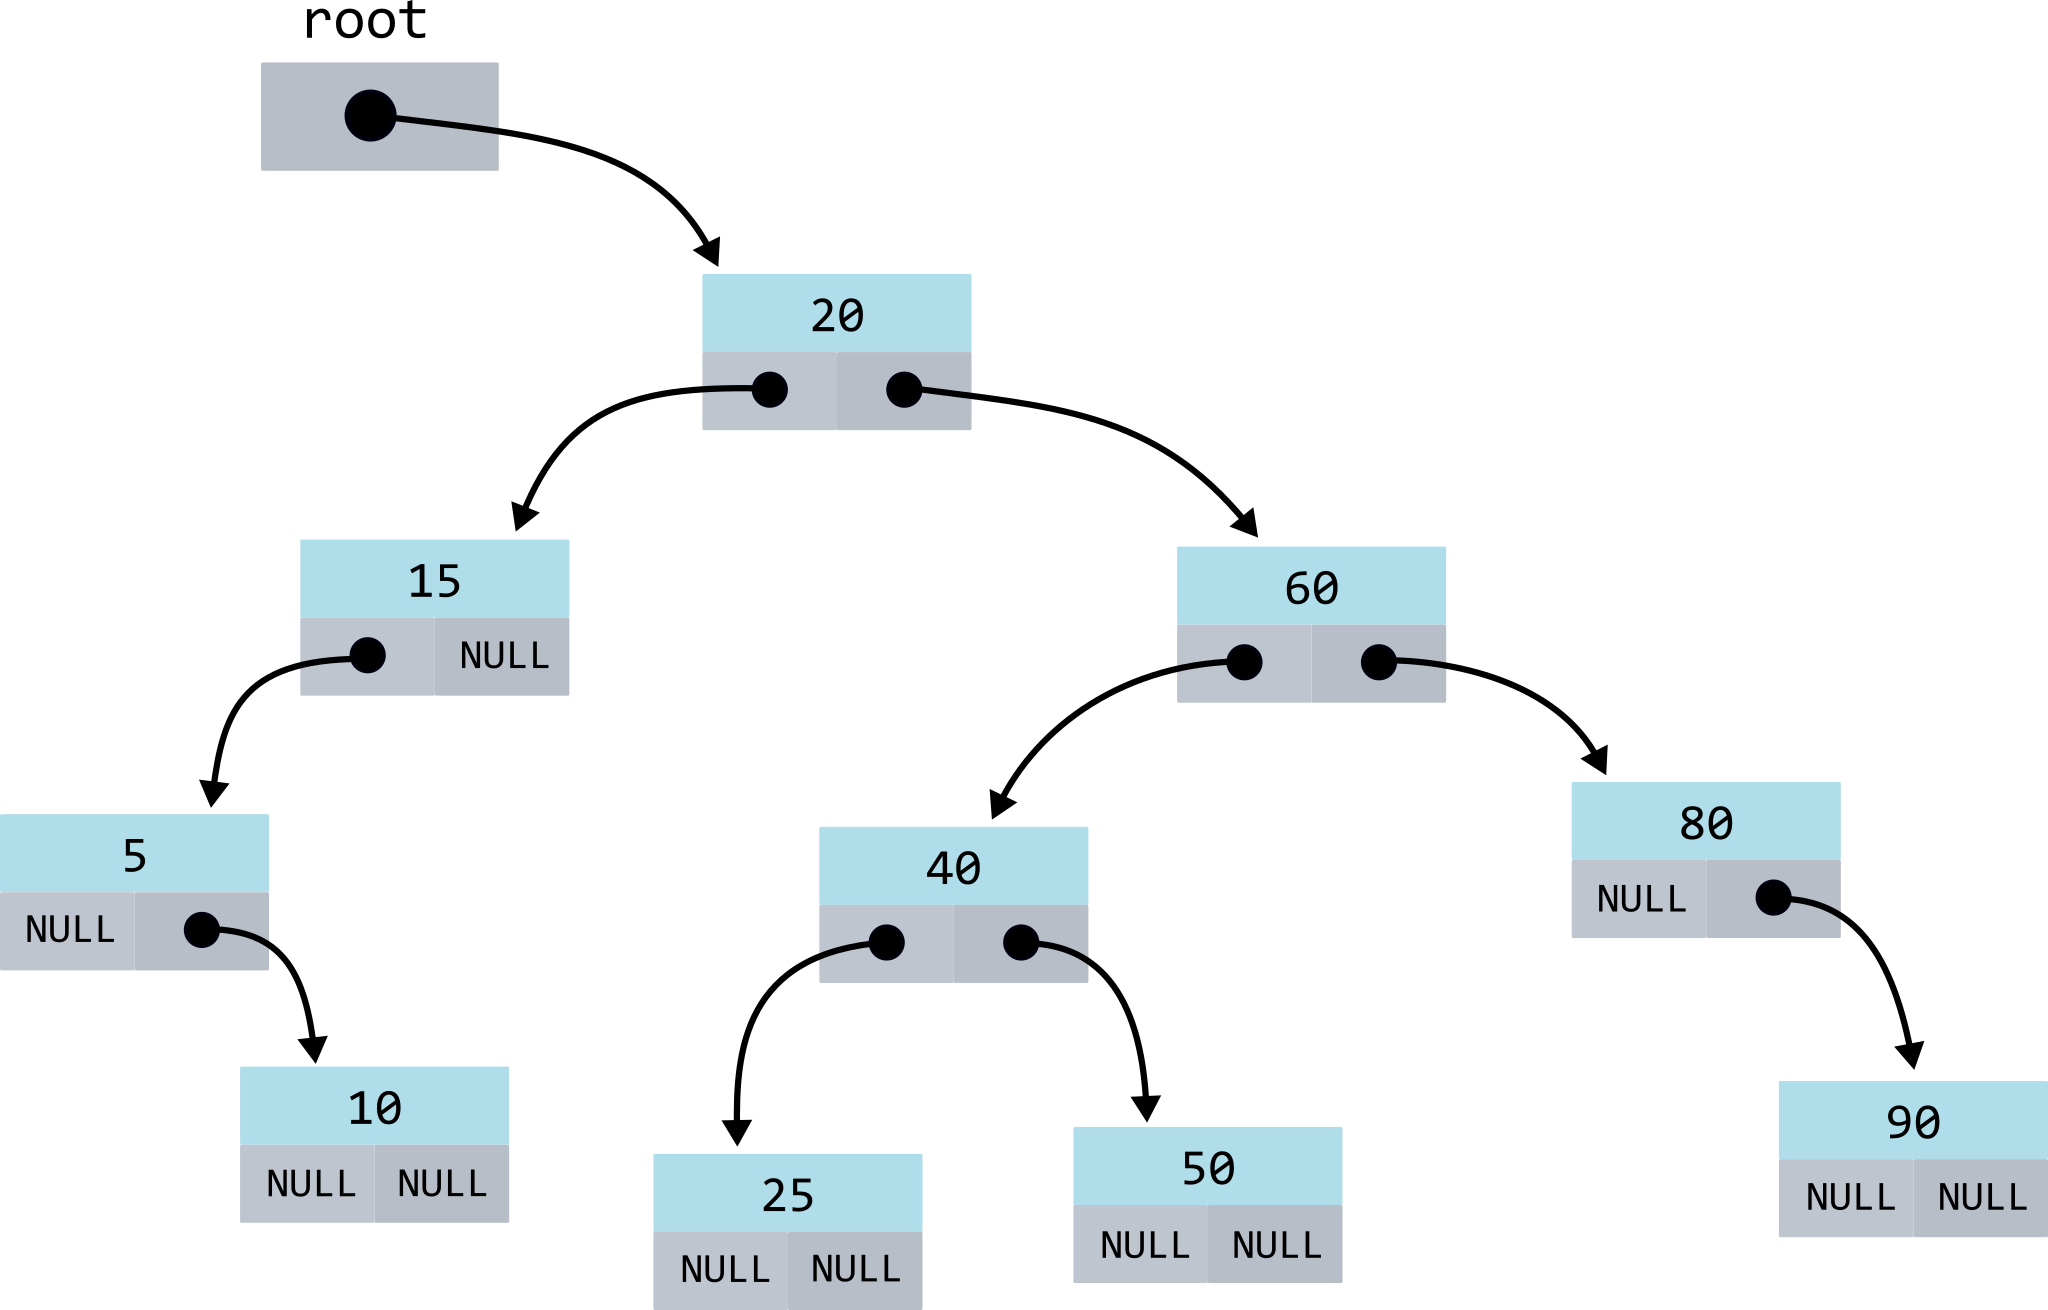
\includegraphics[scale=0.6]{images/tree/bst.png}
\end{center}
\end{frame}


\begin{frame}[fragile]
\frametitle{Вставка элемента в бинарное дерево поиска}
\begin{center}
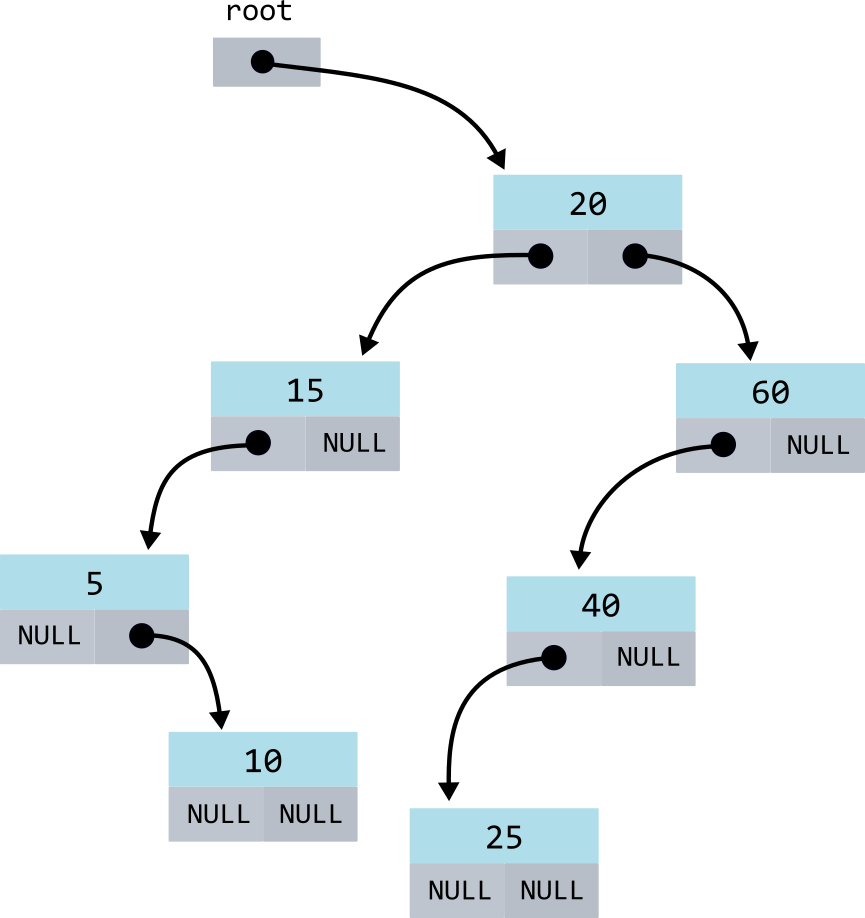
\includegraphics[scale=0.8]{images/tree/codetree/codetree0.png}
\end{center}
\end{frame}


\begin{frame}[fragile]
\frametitle{Вставка элемента в бинарное дерево поиска}
\begin{center}
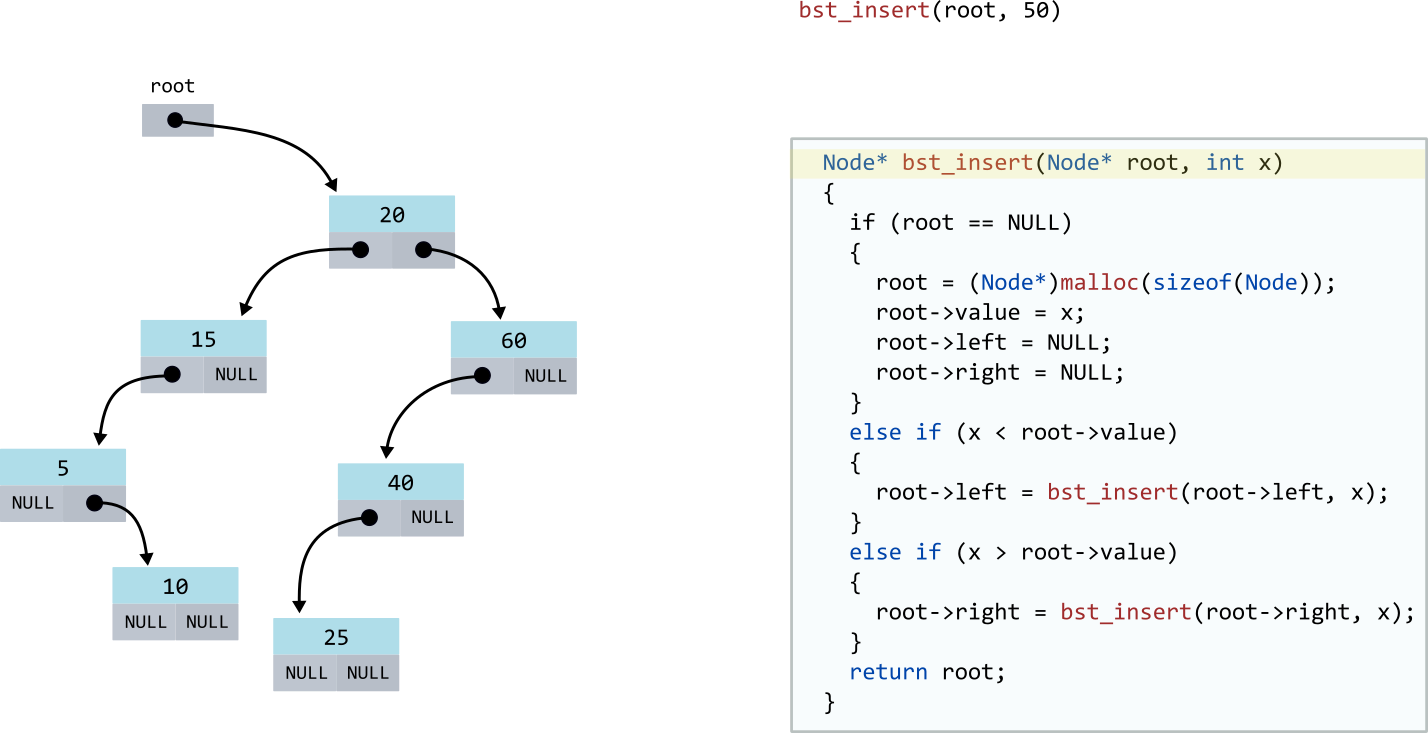
\includegraphics[scale=0.6]{images/tree/codetree/codetree1.png}
\end{center}
\end{frame}

\begin{frame}[fragile]
\frametitle{Вставка элемента в бинарное дерево поиска}
\begin{center}
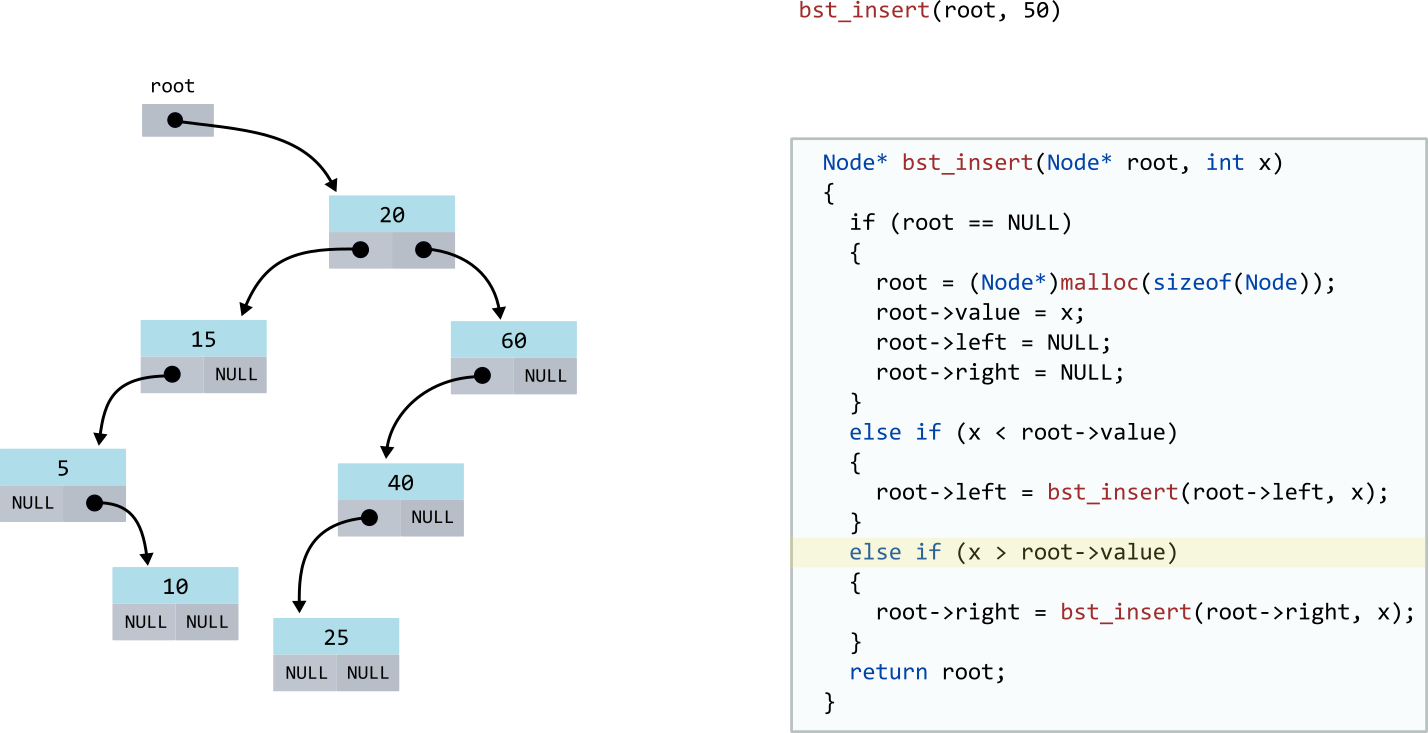
\includegraphics[scale=0.6]{images/tree/codetree/codetree2.png}
\end{center}
\end{frame}
\begin{frame}[fragile]
\frametitle{Вставка элемента в бинарное дерево поиска}
\begin{center}
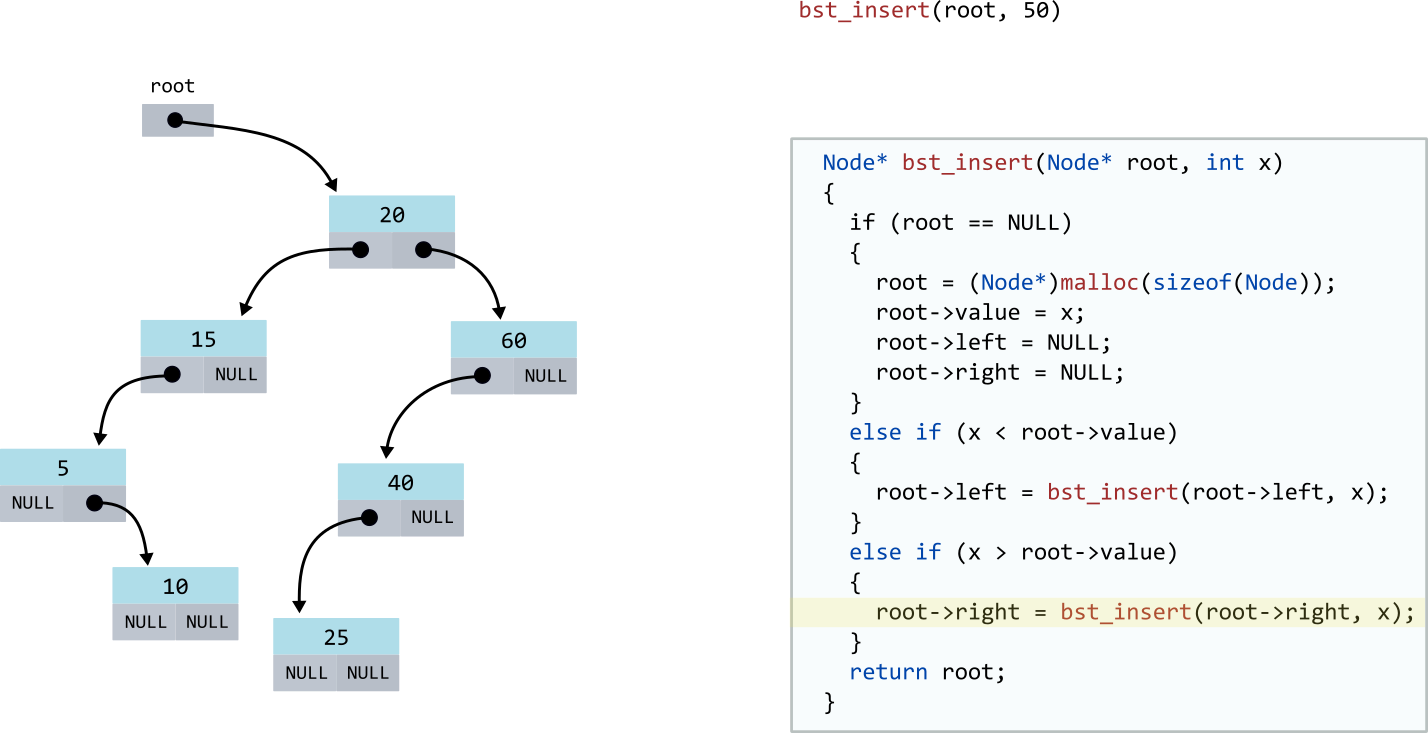
\includegraphics[scale=0.6]{images/tree/codetree/codetree3.png}
\end{center}
\end{frame}
\begin{frame}[fragile]
\frametitle{Вставка элемента в бинарное дерево поиска}
\begin{center}
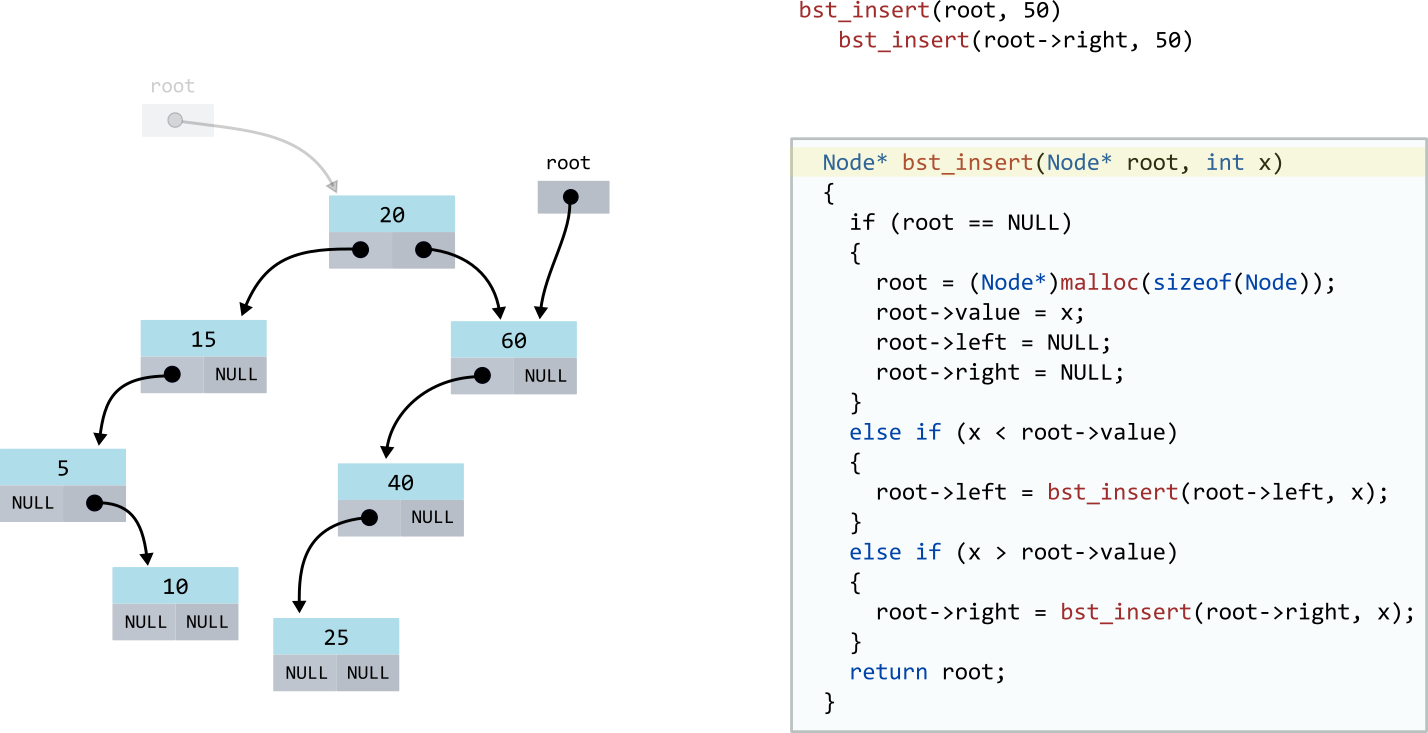
\includegraphics[scale=0.6]{images/tree/codetree/codetree4.png}
\end{center}
\end{frame}
\begin{frame}[fragile]
\frametitle{Вставка элемента в бинарное дерево поиска}
\begin{center}
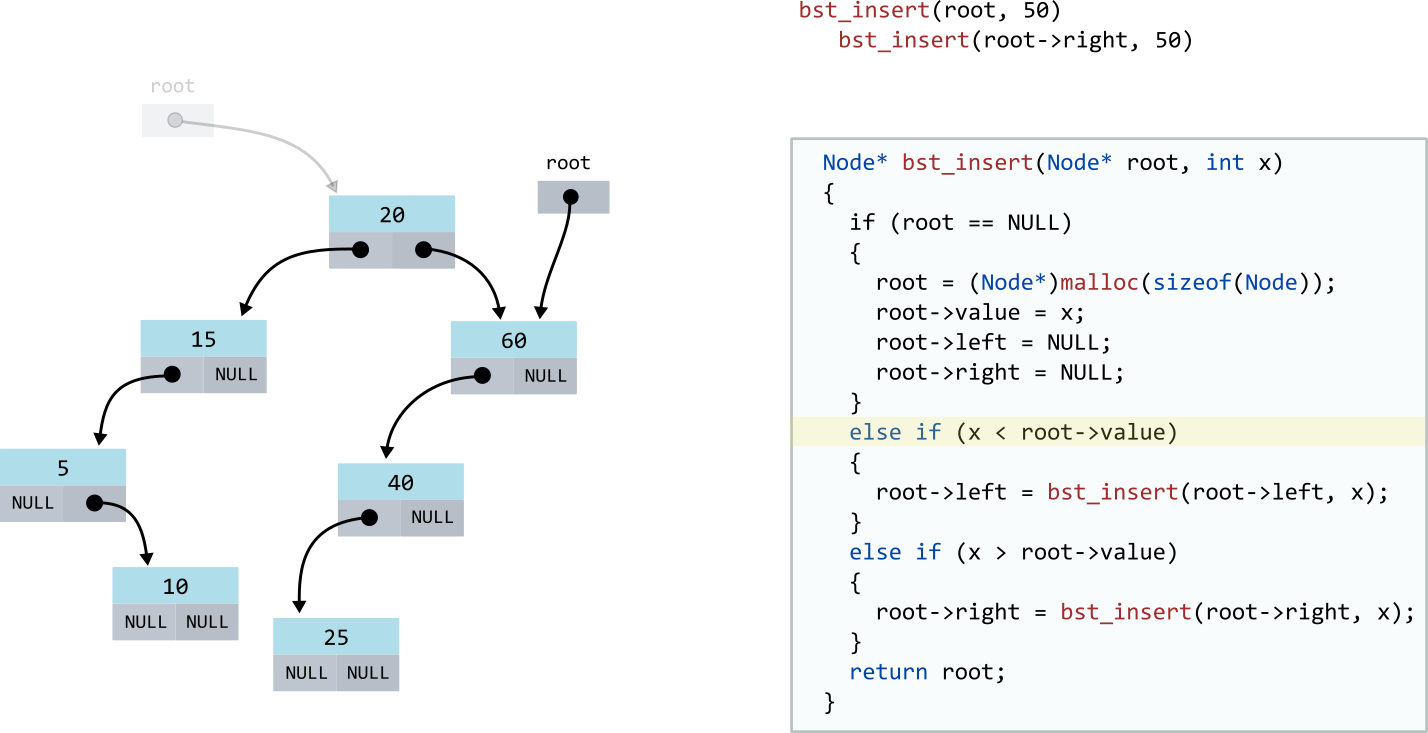
\includegraphics[scale=0.6]{images/tree/codetree/codetree5.png}
\end{center}
\end{frame}
\begin{frame}[fragile]
\frametitle{Вставка элемента в бинарное дерево поиска}
\begin{center}
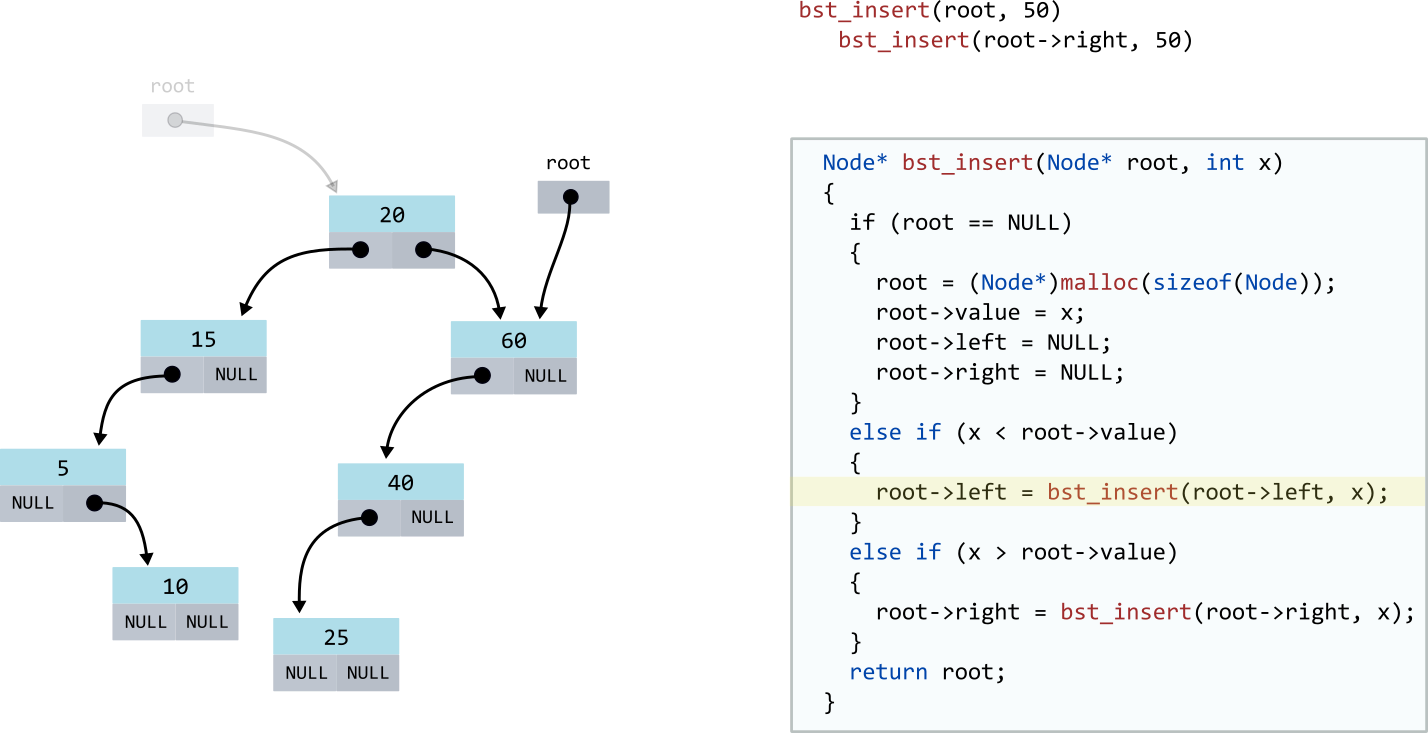
\includegraphics[scale=0.6]{images/tree/codetree/codetree6.png}
\end{center}
\end{frame}
\begin{frame}[fragile]
\frametitle{Вставка элемента в бинарное дерево поиска}
\begin{center}
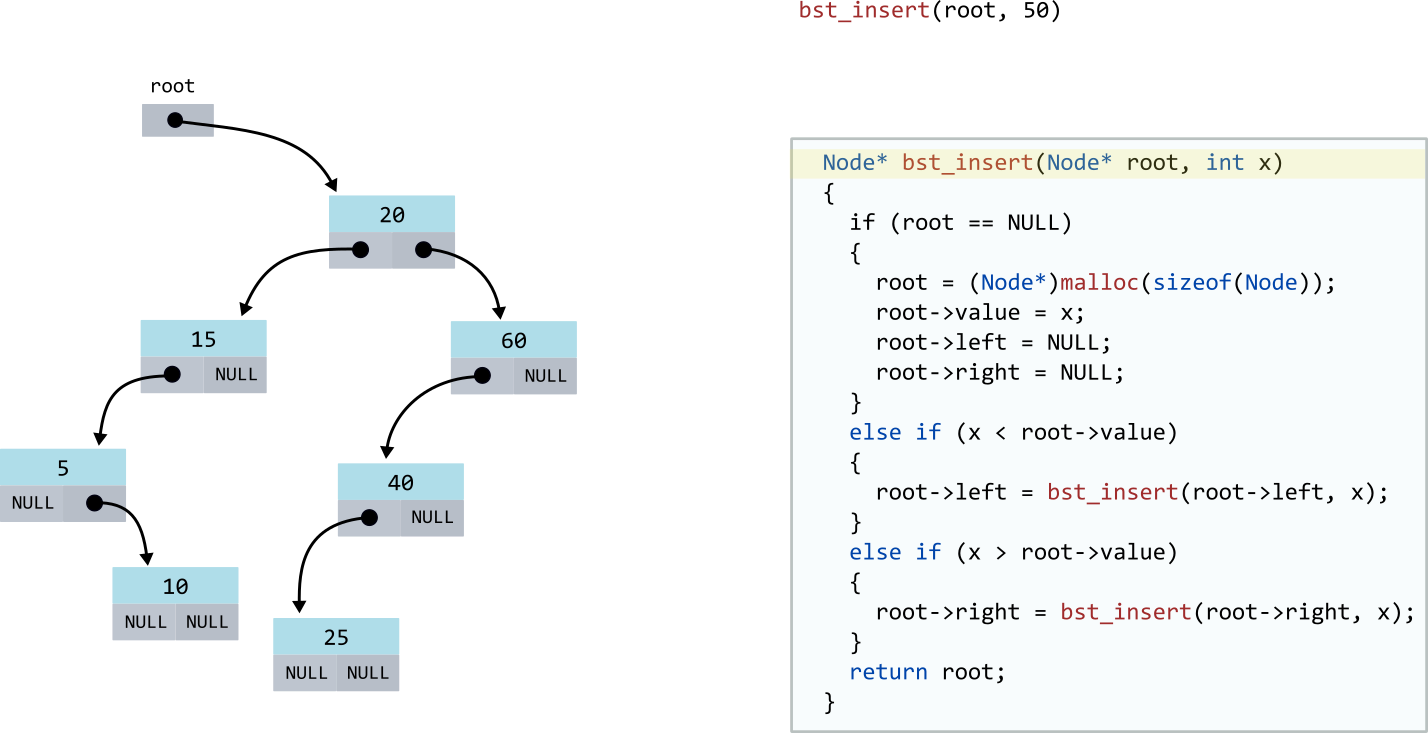
\includegraphics[scale=0.6]{images/tree/codetree/codetree1.png}
\end{center}
\end{frame}
\begin{frame}[fragile]
\frametitle{Вставка элемента в бинарное дерево поиска}
\begin{center}
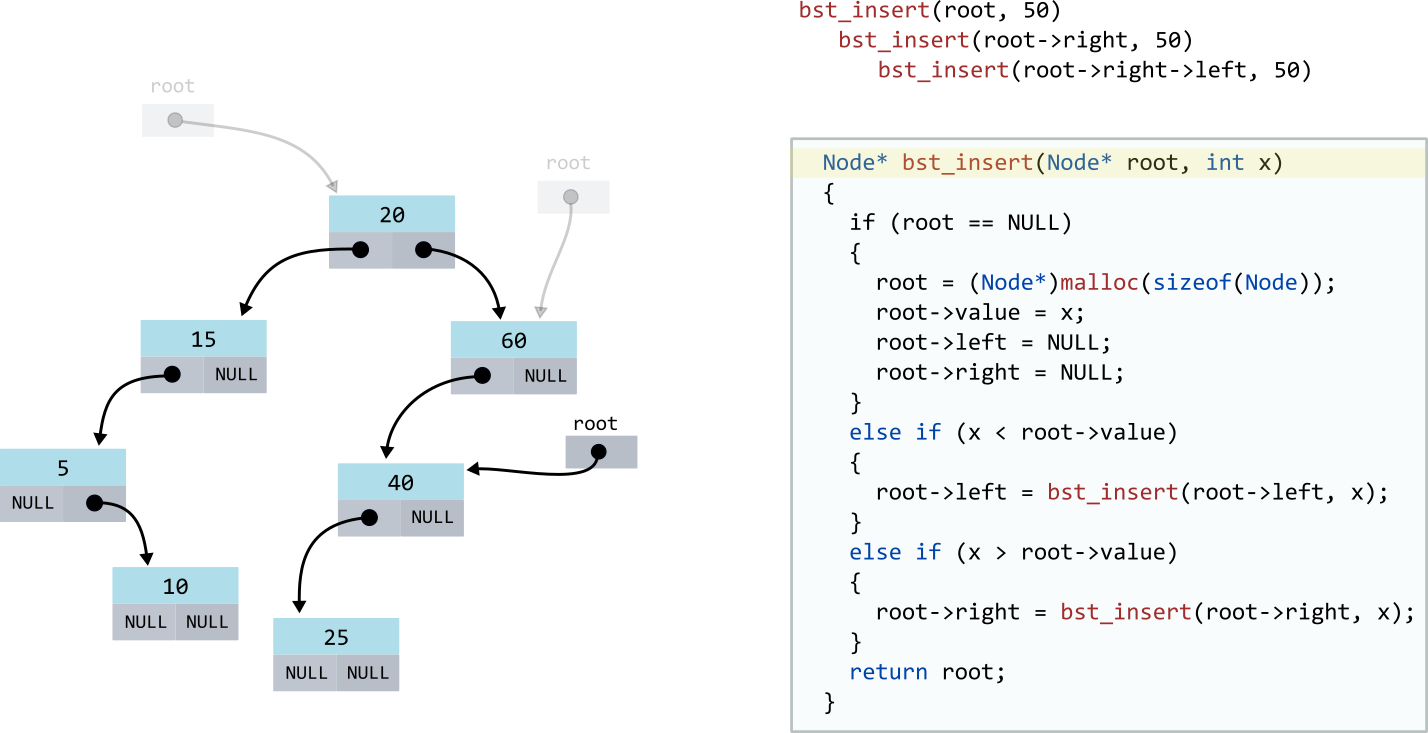
\includegraphics[scale=0.6]{images/tree/codetree/codetree7.png}
\end{center}
\end{frame}
\begin{frame}[fragile]
\frametitle{Вставка элемента в бинарное дерево поиска}
\begin{center}
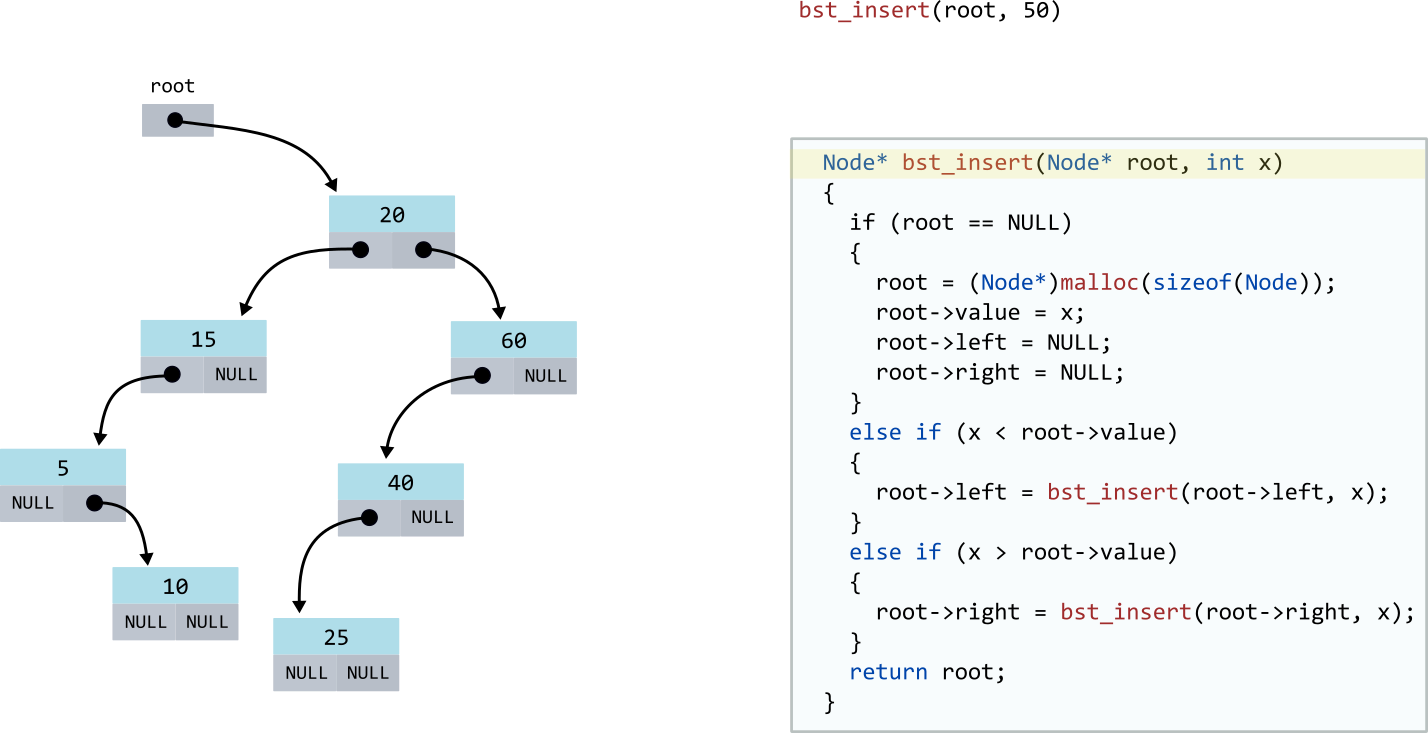
\includegraphics[scale=0.6]{images/tree/codetree/codetree1.png}
\end{center}
\end{frame}
\begin{frame}[fragile]
\frametitle{Вставка элемента в бинарное дерево поиска}
\begin{center}
\includegraphics[scale=0.6]{images/tree/codetree/codetree8.png}
\end{center}
\end{frame}
\begin{frame}[fragile]
\frametitle{Вставка элемента в бинарное дерево поиска}
\begin{center}
\includegraphics[scale=0.6]{images/tree/codetree/codetree9.png}
\end{center}
\end{frame}
\begin{frame}[fragile]
\frametitle{Вставка элемента в бинарное дерево поиска}
\begin{center}
\includegraphics[scale=0.6]{images/tree/codetree/codetree10.png}
\end{center}
\end{frame}
\begin{frame}[fragile]
\frametitle{Вставка элемента в бинарное дерево поиска}
\begin{center}
\includegraphics[scale=0.6]{images/tree/codetree/codetree11.png}
\end{center}
\end{frame}
\begin{frame}[fragile]
\frametitle{Вставка элемента в бинарное дерево поиска}
\begin{center}
\includegraphics[scale=0.6]{images/tree/codetree/codetree12.png}
\end{center}
\end{frame}
\begin{frame}[fragile]
\frametitle{Вставка элемента в бинарное дерево поиска}
\begin{center}
\includegraphics[scale=0.6]{images/tree/codetree/codetree13.png}
\end{center}
\end{frame}
\begin{frame}[fragile]
\frametitle{Вставка элемента в бинарное дерево поиска}
\begin{center}
\includegraphics[scale=0.6]{images/tree/codetree/codetree14.png}
\end{center}
\end{frame}
\begin{frame}[fragile]
\frametitle{Вставка элемента в бинарное дерево поиска}
\begin{center}
\includegraphics[scale=0.6]{images/tree/codetree/codetree15.png}
\end{center}
\end{frame}
\begin{frame}[fragile]
\frametitle{Вставка элемента в бинарное дерево поиска}
\begin{center}
\includegraphics[scale=0.6]{images/tree/codetree/codetree16.png}
\end{center}
\end{frame}
\begin{frame}[fragile]
\frametitle{Вставка элемента в бинарное дерево поиска}
\begin{center}
\includegraphics[scale=0.6]{images/tree/codetree/codetree14.png}
\end{center}
\end{frame}
\begin{frame}[fragile]
\frametitle{Вставка элемента в бинарное дерево поиска}
\begin{center}
\includegraphics[scale=0.6]{images/tree/codetree/codetree17.png}
\end{center}
\end{frame}
\begin{frame}[fragile]
\frametitle{Вставка элемента в бинарное дерево поиска}
\begin{center}
\includegraphics[scale=0.6]{images/tree/codetree/codetree18.png}
\end{center}
\end{frame}
\begin{frame}[fragile]
\frametitle{Вставка элемента в бинарное дерево поиска}
\begin{center}
\includegraphics[scale=0.6]{images/tree/codetree/codetree19.png}
\end{center}
\end{frame}
\begin{frame}[fragile]
\frametitle{Вставка элемента в бинарное дерево поиска}
\begin{center}
\includegraphics[scale=0.6]{images/tree/codetree/codetree20.png}
\end{center}
\end{frame}
\begin{frame}[fragile]
\frametitle{Вставка элемента в бинарное дерево поиска}
\begin{center}
\includegraphics[scale=0.6]{images/tree/codetree/codetree21.png}
\end{center}
\end{frame}
\begin{frame}[fragile]
\frametitle{Вставка элемента в бинарное дерево поиска}
\begin{center}
\includegraphics[scale=0.6]{images/tree/codetree/codetree22.png}
\end{center}
\end{frame}

\begin{frame}[fragile]
\frametitle{Несбалансированное дерево поиска}
\begin{center}
\includegraphics[scale=0.6]{images/tree/unbalanced_tree.png}
\end{center}
\end{frame}

\begin{frame}[fragile]
\frametitle{Сбалансированное дерево поиска}
\begin{center}
\includegraphics[scale=0.6]{images/tree/balanced_tree.png}
\end{center}
\end{frame}

\begin{frame}[fragile]
\frametitle{Самобалансирующееся дерево поиска (AVL)}
\begin{center}
\includegraphics[scale=0.4]{images/tree/avl_example.png}
\end{center}
\end{frame}


\section{Дерево поиска в стандартной библиотеке C++.}

\begin{frame}[fragile]
\frametitle{Множества \texttt{std::set} и \texttt{std::multiset}}
\begin{itemize}
\item \texttt{std::set} - это упорядоченное множество (как правило реализовано с помощью самобалансирующегося
дерева поиска)
\begin{lstlisting}
std::set a {10, 20, 30, 40, 50};
a.insert(60);
\end{lstlisting}

\item \texttt{std::multiset} - это упорядоченное множество, которое может хранить дубликаты.
\begin{lstlisting}
std::multiset a {10, 20, 10, 20, 50};
a.insert(50);
\end{lstlisting}
\end{itemize}
\end{frame}


\begin{frame}[fragile]
\frametitle{Множества \texttt{std::set}}
\begin{lstlisting}
std::set<std::string> s {"Cat", "Mouse", "Dog"};
s.insert("Bat");
s.insert("Elephant");
\end{lstlisting}

\begin{center}
\includegraphics[scale=0.8]{images/tree/bst_set_string.png}
\end{center}
\end{frame}


\begin{frame}[fragile]
\frametitle{Словарь \texttt{std::map}}
\begin{lstlisting}
std::map<std::string, int> m{{"Cat",20},{"Mouse", 3}};
m["Dog"] = 30;
m["Bat"] = 2;
m["Elephant"] = 80;
\end{lstlisting}
\begin{center}
\includegraphics[scale=0.7]{images/tree/bst_dict.png}
\end{center}
\end{frame}


\section{Хеш-таблица}
\begin{frame}[fragile]
\frametitle{Множество \texttt{std::unordered\_set}}
\begin{itemize}
\item \texttt{std::unordered\_set} - это неупорядоченное множество (как правило реализовано с помощью хеш-таблицы)
\begin{lstlisting}
std::unordered_set a {10, 20, 30, 40, 50};
a.insert(60);
\end{lstlisting}

\item \texttt{std::unordered\_multiset} - это неупорядоченное множество  (как правило реализованое с помощью хеш-таблицы), которое может хранить дубликаты.
\begin{lstlisting}
std::unordered_multiset a {10, 20, 10, 20, 50};
a.insert(50);
\end{lstlisting}
\end{itemize}
\end{frame}


\begin{frame}[fragile]
\frametitle{Множество \texttt{std::unordered\_set}}
\begin{lstlisting}
std::unordered_set<std::string> s {"Cat", "Mouse"};
s.insert("Dog");
s.insert("Bat");
s.insert("Elephant");
s.insert("Axolotl");
s.insert("Tiger");
\end{lstlisting}
\end{frame}

\begin{frame}[fragile]
\frametitle{Множество \texttt{std::unordered\_set}}
\begin{center}
\includegraphics[scale=0.7]{images/hashtable/hashtable_set.png}
\end{center}
\end{frame}


\begin{frame}[fragile]
\frametitle{Словарь \texttt{std::unordered\_map}}
\begin{lstlisting}
std::unordered_map<std::string, int> m {{"Cat", 20}};
m["Mouse"] = 2;
m["Dog"] = 30;
m["Bat"] = 2;
m["Elephant"] = 80;
m["Axolotl"] = 120;
m["Tiger"] = 50;
\end{lstlisting}
\end{frame}

\begin{frame}[fragile]
\frametitle{Словарь \texttt{std::unordered\_map}}
\begin{center}
\includegraphics[scale=0.7]{images/hashtable/hashtable_map.png}
\end{center}
\end{frame}

\section{Контейнеры}

\begin{frame}[fragile]
\frametitle{Контейнеры}
\begin{center}
\begin{tabular}{ l | l }
 контейнер & описание и основные свойства \\ \hline
 \texttt{std::array} &  Массив фиксированного размера \\ \\ \hline

 \texttt{std::vector} & Динамический массив \\
                      & Все элементы лежат вплотную друг к другу \\
                      & Есть доступ по индексу за $O(1)$ \\ \\ \hline
 \texttt{std::list} & Двусвязный список \\
                    & Вставка/удаление элементов за $O(1)$ \\ &если есть итератор на элемент \\ \\ \hline
 \texttt{std::forward\_list} & Односвязный список \\
                     & Вставка/удаление элементов за $O(1)$ \\ &если есть итератор на предыдущий элемент\\ \\ \hline
                     
\end{tabular}
\end{center}
\end{frame}

\begin{frame}[fragile]
\frametitle{Контейнеры}
\begin{center}
\begin{tabular}{ l | l }
 \texttt{std::set} & Реализация множества на основе сбалансированного дерева  \\
				   & поиска. Хранит элементы без дубликатов, в отсортированном \\
                   & виде. Поиск/вставка/удаление элементов за $O(\log(N))$ \\ \\ \hline
 \texttt{std::map} & Реализация словаря на основе сбалансированного дерева  \\
				   & поиска. Хранит пары ключ-значения без дубликатов ключей, \\
				   & в отсортированном виде\\
                   & Поиск/вставка/удаление элементов за $O(\log(N))$ \\ \\ \hline
\end{tabular}
\end{center}
\end{frame}    
          
\begin{frame}[fragile]
\frametitle{Контейнеры}
\begin{center}
\begin{tabular}{ l | l }
 \texttt{std::unordered\_set} & Реализация множества на основе хеш-таблицы \\
				   & Хранит элементы без дубликатов, \\ &в произвольном порядке\\
                   & Поиск/вставка/удаление элементов за $O(1)$ \\ &в среднем \\ \\ \hline
 \texttt{std::unordered\_map} & Реализация словаря на основе хеш-таблицы \\
				   & Хранит пары ключ-значения без дубликатов \\&ключей,в произвольном порядке\\
                   & Поиск/вставка/удаление элементов за $O(1)$ \\&в среднем  \\ \\ \hline
 \texttt{std::multiset} & То же самое, что \texttt{std::set}, но может хранить \\&дублированные значения \\ \\ \hline
\end{tabular}
\end{center}
\end{frame}
\end{document}